\documentclass{mpaper}
\usepackage{multirow}
\usepackage{graphics}
\usepackage{float}
\usepackage{pdfpages}
\usepackage{graphicx}
\usepackage{subcaption}
\usepackage[bottom]{footmisc}

\captionsetup[figure]{font={bf},skip=0.6\baselineskip, labelsep=period}
\captionsetup[table]{font={bf},skip=0.6\baselineskip, labelsep=period}


\begin{document}
\title{Insights into Electrotactile Feedback: Parameters and User Preferences}
\author{Aaron Milne}
\matricnum{2466574M}

\maketitle

\begin{abstract}
Electrotactile feedback, a novel extension to tactile interaction, offers distinct advantages over traditional haptic modalities such as vibrotactile feedback. Despite its potential, the optimal application of electrotactile feedback to everyday devices remains uncertain. This paper aims to uncover ideal values for the primary parameters affecting electrotactile signals — pulse-width $({\mu}s)$, frequency (pulses per second), and amplitude (mA) — across various contexts. Furthermore, we will look more qualitatively at user opinions of electrotactile feedback.

Three user evaluations were conducted. Initially, participants adjusted the aforementioned parameters until the signal experienced through interaction with various interface widgets felt appropriate. Subsequently, presets were established based on these findings and a separate group of users selected their preferred preset, while interacting with the same widgets. Finally, a qualitative approach was employed, with users completing simple number and phrase entry tasks, whilst experiencing electrotactile signals. Half of the tasks were performed at the intensity of the best-performing presets from before, while the remainder produced no electrotactile feedback.

The first experiment clarified the range of suitable values, with results falling within a clear cluster. The second showed that the median preset - selected deterministically by taking averages from the results of phase one - was the most popular. It also showed that the further we moved from the centre of the cluster, the less popular the presets became. Finally, the third evaluation demonstrated some efficiency advantages of electrotactile feedback, when completing simple tasks. Moreover, it provided an understanding of the opinions surrounding this method of feedback.

These results shed light on effective strategies for implementing electrotactile feedback into user interfaces, paving the way for its broader integration into applications and devices. 
\end{abstract}

\section{Introduction}\label{sec:intro}

Electrotactile feedback represents a novel branch of tactile interaction. In contrast to vibrotactile feedback - the most common form of haptics - which utilises vibrations to convey responses to its users; electrotactile feedback instead employs a small electrical current to directly provide feedback to the skin of a user.

The strength associated with electrotactile signals is certainly an area of key importance when it comes to usability. Too weak and users will not perceive the sensation, yet too strong and the shock becomes unpleasant. The strength of said cue is controlled by altering three main parameters: pulse-width (${\mu}s$), frequency (pulses per second), and amplitude (mA). The first indicates the duration of each pulse and the frequency determines how many pulses occur in one second. The amplitude measures how much electrical current each pulse carries, which when combined with pulse-width, translates to the intensity of each cue.

Figure \ref{pulse-struc} "shows the basic structure of the electrotactile signal, and the parameters that can be manipulated to encode information in an electrotactile cue." \cite{10.1145/3491102.3501863} As can be visualised here, the amplitude of the signal represents the height, or energy, that each pulse carries. Combining this with pulse-width, ie. how long each pulse lasts, denotes the intensity of each signal. The pulse frequency, as explored by Alotaibi \emph{et al.} and Yoshimoto \emph{et al.} represents how many pulses occur in a single second and can be an indicator of electrotactile roughness \cite{10.1145/3491102.3501863, yoshimoto}. It should be noted that Figure \ref{pulse-struc} also draws attention to the 'refresh period' and 'pulse interval' parameters. While these parameters could also be tuned, they were beyond the scope of this paper. They do, however, represent promising areas for additional research.

\begin{figure}
    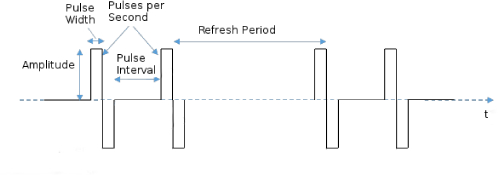
\includegraphics[scale=0.4]{images/chi22-46-fig2.jpg}
    \caption{\label{pulse-struc} "The structure of a biphasic electrotactile stimulus. The X axis is time, the Y axis is amplitude. The electrotactile stimulus increases from 0 (mA) to a specific value for some time and returns to 0. That time is the pulse width. The time between each stimulus is the pulse interval. The number of electrotactile pulses in a second is the pulse frequency (pulses per second, PPS)." Adapted from Alotaibi et al. sec. 2.1. \cite{10.1145/3491102.3501863}}
\end{figure}

The primary objective of this paper was to further our understanding of how these parameters affect user perceptions of electrotactile cues. Furthermore, we aimed to discover an ideal range of values for said parameters, such that the electrotactile signals experienced by users were comfortable and appropriate. What was considered appropriate was hypothesised to depend on the type of interaction undertaken by the participants. The first two evaluations set out in this paper focus on this objective. The first allowed users to choose parameter values from a continuous range, while the second expanded on this by getting them to choose their favourite from five discrete presets.

A secondary aim was to gather more general, qualitative, information on the suitability, effectiveness and comfort of electrotactile feedback. This was to expand on our current knowledge of applying electrotactile feedback, in user-friendly ways, to everyday devices for the future. The purpose of the final evaluation outlined in this paper was to achieve this. We obtained this data by comparing the accuracy and time taken to complete short tasks, as well as analysing the results of an extensive questionnaire.

The significance of research in this area becomes apparent when considering the ever-increasing reliance we, as humans, place on our mobile devices. Non-visual methods of computer feedback are essential for notifying us of events, reminders, incoming calls and the many other alerts we receive daily. This becomes particularly important in scenarios where visual cues are impractical; such as when in meetings, or working. A significant quantity of research investigating viable alternatives to visual methods of feedback has been undertaken previously \cite{10.1145/1322192.1322222, vibro_wearables, blind_study}, however, minimal research has been completed regarding the refinement of electrotactile feedback. Investigating solutions to this, such that it becomes a pleasant and usable experience for users is, therefore, a sensible heading to follow. 

\section{Background}
\subsection{Electrotactile Feedback}
Electrotactile feedback operates by supplying a small electrical current across the skin. There are four types of mechanoreceptors present within human skin \cite{10.1145/3491102.3501863, hand_book}. These mechanoreceptors are each responsible for detecting various actions impacting the skin. Each is sensitive to its unique range of frequencies and produces stimuli of varying sensations. Electrotactile Feedback has been found to trigger mechanoreceptors correlating to sensations of itchiness and touch \cite{9086329, artificial_skin}. Therefore, rendering it a plausible modality of tactile feedback.

Previous work produced by Stanke \emph{et al} has contributed widely to this area of tactile interaction. During a study of theirs \cite{rings_and_watch}, they put electrotactile feedback against the more common vibrotactile feedback, with a focus particularly on wearable devices like watches and rings. These are some of the most likely use cases for electrotactile feedback, due to a direct contact point on the skin being required. They conclude that electrotactile feedback produces much more localised sensation around the wrist versus vibrotactile methods. Furthermore, they found that electrotactile cues can produce sensations away from the contact point. They used this information to look at suitable devices and patterns that could be used for notifications. They found slightly better results using electrotactile methods in this scenario. They also state that when it came to rings, participants found this type of feedback more comfortable. 

\subsection{Limitations of Visual Feedback Modalities}
The demand for electrotactile feedback - rather, non-visual feedback methods in general - becomes apparent when we consider the cases where visual feedback methods are inappropriate. Hoggan \emph{et al.} \cite{10.1145/1322192.1322222} outline some situations where visual methods of feedback are inappropriate - such as when in a meeting, or listening to music.

Another limitation of visual feedback methods becomes apparent when we consider making computer interactions accessible for blind and partially sighted users. Metatla \emph{et al} \cite{blind_study} highlight this limitation, and put forward a solution to this by creating voice user interfaces (VUIs) in the context of schools. Their method proved to aid the feeling of inclusion among visually impaired children within their school. 

\subsection{Alternative Tactile Feedback Approaches}
A solution to the limitations mentioned above comes in the form of tactile interaction. This form of feedback includes "devices that render a precept of the cutaneous sense", cutaneous being "sensations [that] come from the skin [which] can include vibration, touch, pressure,
temperature, and texture" \cite{multimodal_feedback}. The most common of which is vibrotactile feedback. This term describes using vibrations to convey signals to users. 

There has been a lot of research into the vibrotactile modality, including that of Matscheko \emph{et al}. Their study investigated how the positioning of tactors in wearable devices affected the alertness of unsuspecting users, receiving notifications \cite{vibro_wearables}. The study proved that arranging the vibrations around participants' wrists yielded an increase in information transfer versus positioning these vibrations in the watch face. This highlights the importance of positioning and configuration of tactile feedback - applying also to our study on electrotactile interaction.

Tactile feedback comes in many other forms: thermal feedback and pressure-based, deformable interaction to name just two, and are outlined by Freeman \emph{et al} \cite{multimodal_feedback}. Each of these methodologies has its advantages and drawbacks across different situations. 

\subsection{Benefits of  Electrotactile Feedback}
Electrotactile feedback brings many benefits over the alternative tactile modalities mentioned previously. For example, comparing electrotactile to vibrotactile methods, the actuators used by electrotactile methods are thin, light and durable. Furthermore, they are much more energy efficient than vibrotactile motors - providing an environmental advantage. They are also more responsive, increasing the range of potential use cases. \cite{Alotaibi2023} 

In another article, produced by Duente \emph{et al}. \cite{duente2023colorful}, it was found that unlike the monochrome sensation perceived when using vibrotactile feedback, electrotactile feedback can be used to produce "colourful" - rather, a spectrum of - sensations. The work also indicates that the pulse-width and frequency parameters of electrotactile signals control which of these sensations the cue evokes. A table of values is provided to map these values to the emotions felt by users. While we consider this an advantage of electrotactile feedback in the diversity it offers, it does indicate the precision required in designing such systems correctly.

In addition, electrotactile feedback brings a plethora of accessibility advantages as opposed to traditional methods. Stephens-Fripp \emph{et al} in their paper \cite{Stephens-Fripp} look at utilising electrotactile feedback (among other options) in prosthetic hands to advance them closer to their biological counterparts. The paper shows that electrotactile feedback performs well in many situations, particularly when feedback is required from all five fingers, or when grasping an object. 

\pagebreak
\subsection{Electrotactile Intensity and Roughness}
In their research paper \cite{10.1145/3491102.3501863}, Alotaibi \emph{et al}. discuss the various parameters at play in an electrotactile signal. They consider the same parameters as ourselves: pulse-width (${\mu}s$); frequency (PPS) and amplitude (mA). They make clear that the combination of pulse-width and amplitude characteristics indicate the \emph{intensity} of the signal. The paper goes on to investigate how altering the intensity level influences the emotions of urgency, annoyance, valence and arousal. It was found through their first procedure that an increase in intensity led to an increased rating of all but the valence emotion, which decreased.

This paper \cite{10.1145/3491102.3501863} also makes clear the distinction between \emph{intensity} and \emph{roughness}. They reference prior work by Yoshimoto \emph{et al}. \cite{yoshimoto} that shows through their evaluations, that electrotactile roughness is controlled directly through the pulse frequency (PPS) parameter. Alotaibi \emph{et al}. \cite{10.1145/3491102.3501863} then ran a second evaluation, looking at both intensity and pulse frequency in an attempt to quantify how many of their distinguishable intensity-roughness levels could be perceived. The results of their study showed that both the intensity and frequency of electrotactile cues, play a role in the perception of a signal, forming the basis for our evaluations.\\


\section{Setup and Implementation}
\subsection{Software Requirements} \label{software-requirements}
A fundamental component for all evaluations discussed in this paper was the custom application which we developed for the occasion. This application was simple in nature, but modular in design; allowing alterations to be made easily when switching between the different studies. The same app was used as a foundation for all three phases, with minor differences between each of them. The specific requirements for each evaluation are discussed in more detail in their respective sections, however, the underlying functionality of the app was consistent throughout. Allow users to interact with widgets, sending an electrotactile signal as they do so, before recording various metrics specific to the experiment.

The application was created in Python, using Visual Studio, and is available on GitHub \footnote{\url{https://github.com/AaronMilne19/electrotactile-feedback}}. We used Python's Tkinter library \footnote{\url{https://docs.python.org/3/library/tkinter.html}} to build the user interface, this contained the various widgets that the users interacted with, as well as all applicable controls. Driver code for the device was obtained from former research conducted by Alotaibi \emph{et al.} \cite{9086329, 10.1145/3491102.3501863} and was modernized and adapted slightly to work with our application. This code was responsible for interacting with the electrotactile device, at a low level. For example, controlling the strength and sending the signal to the participant.

\subsection{Apparatus}\label{sec:apparaus}
The following apparatus is all which was used across each of the three evaluations discussed in this paper.
\begin{itemize}
    \item A laptop, to run the custom application mentioned in section \ref{software-requirements}.
    \item A USB mouse to interact with the widgets.
    \item MOTIONSTIM 8 Functional electrical stimulator (FES) device - used to produce electrotactile signals. (This is the same device as was used by Alotaibi et al \cite{9086329, 10.1145/3491102.3501863}).
    \item Two Axion 60x30mm self-adhesive electrodes per participant. (These could be reused on other participants, however, new ones were used where available to maximise consistency).
\end{itemize}

Looking at Figure \ref{fig:apparatus}, you can view this apparatus as it was configured during the experiments.

\subsection{Ethics} \label{ethics}
Care was taken to ensure relevant ethics procedures were followed across all studies. Special permission was obtained from the School of Computer Science ethics committee \footnote{\url{https://www.gla.ac.uk/schools/computing/informationforstudents/\#ethicsprocedures}} to perform our experiments, as we were utilising a non-standard device. Before taking part, participants of all evaluations were required to read the provided information sheet, detailing the experiment and any potential risks associated. Subjects were also required to sign a consent form, ensuring that explicit consent was obtained and that those who were pregnant or who had any underlying heart conditions, were excluded.

\begin{figure}
    \centering
    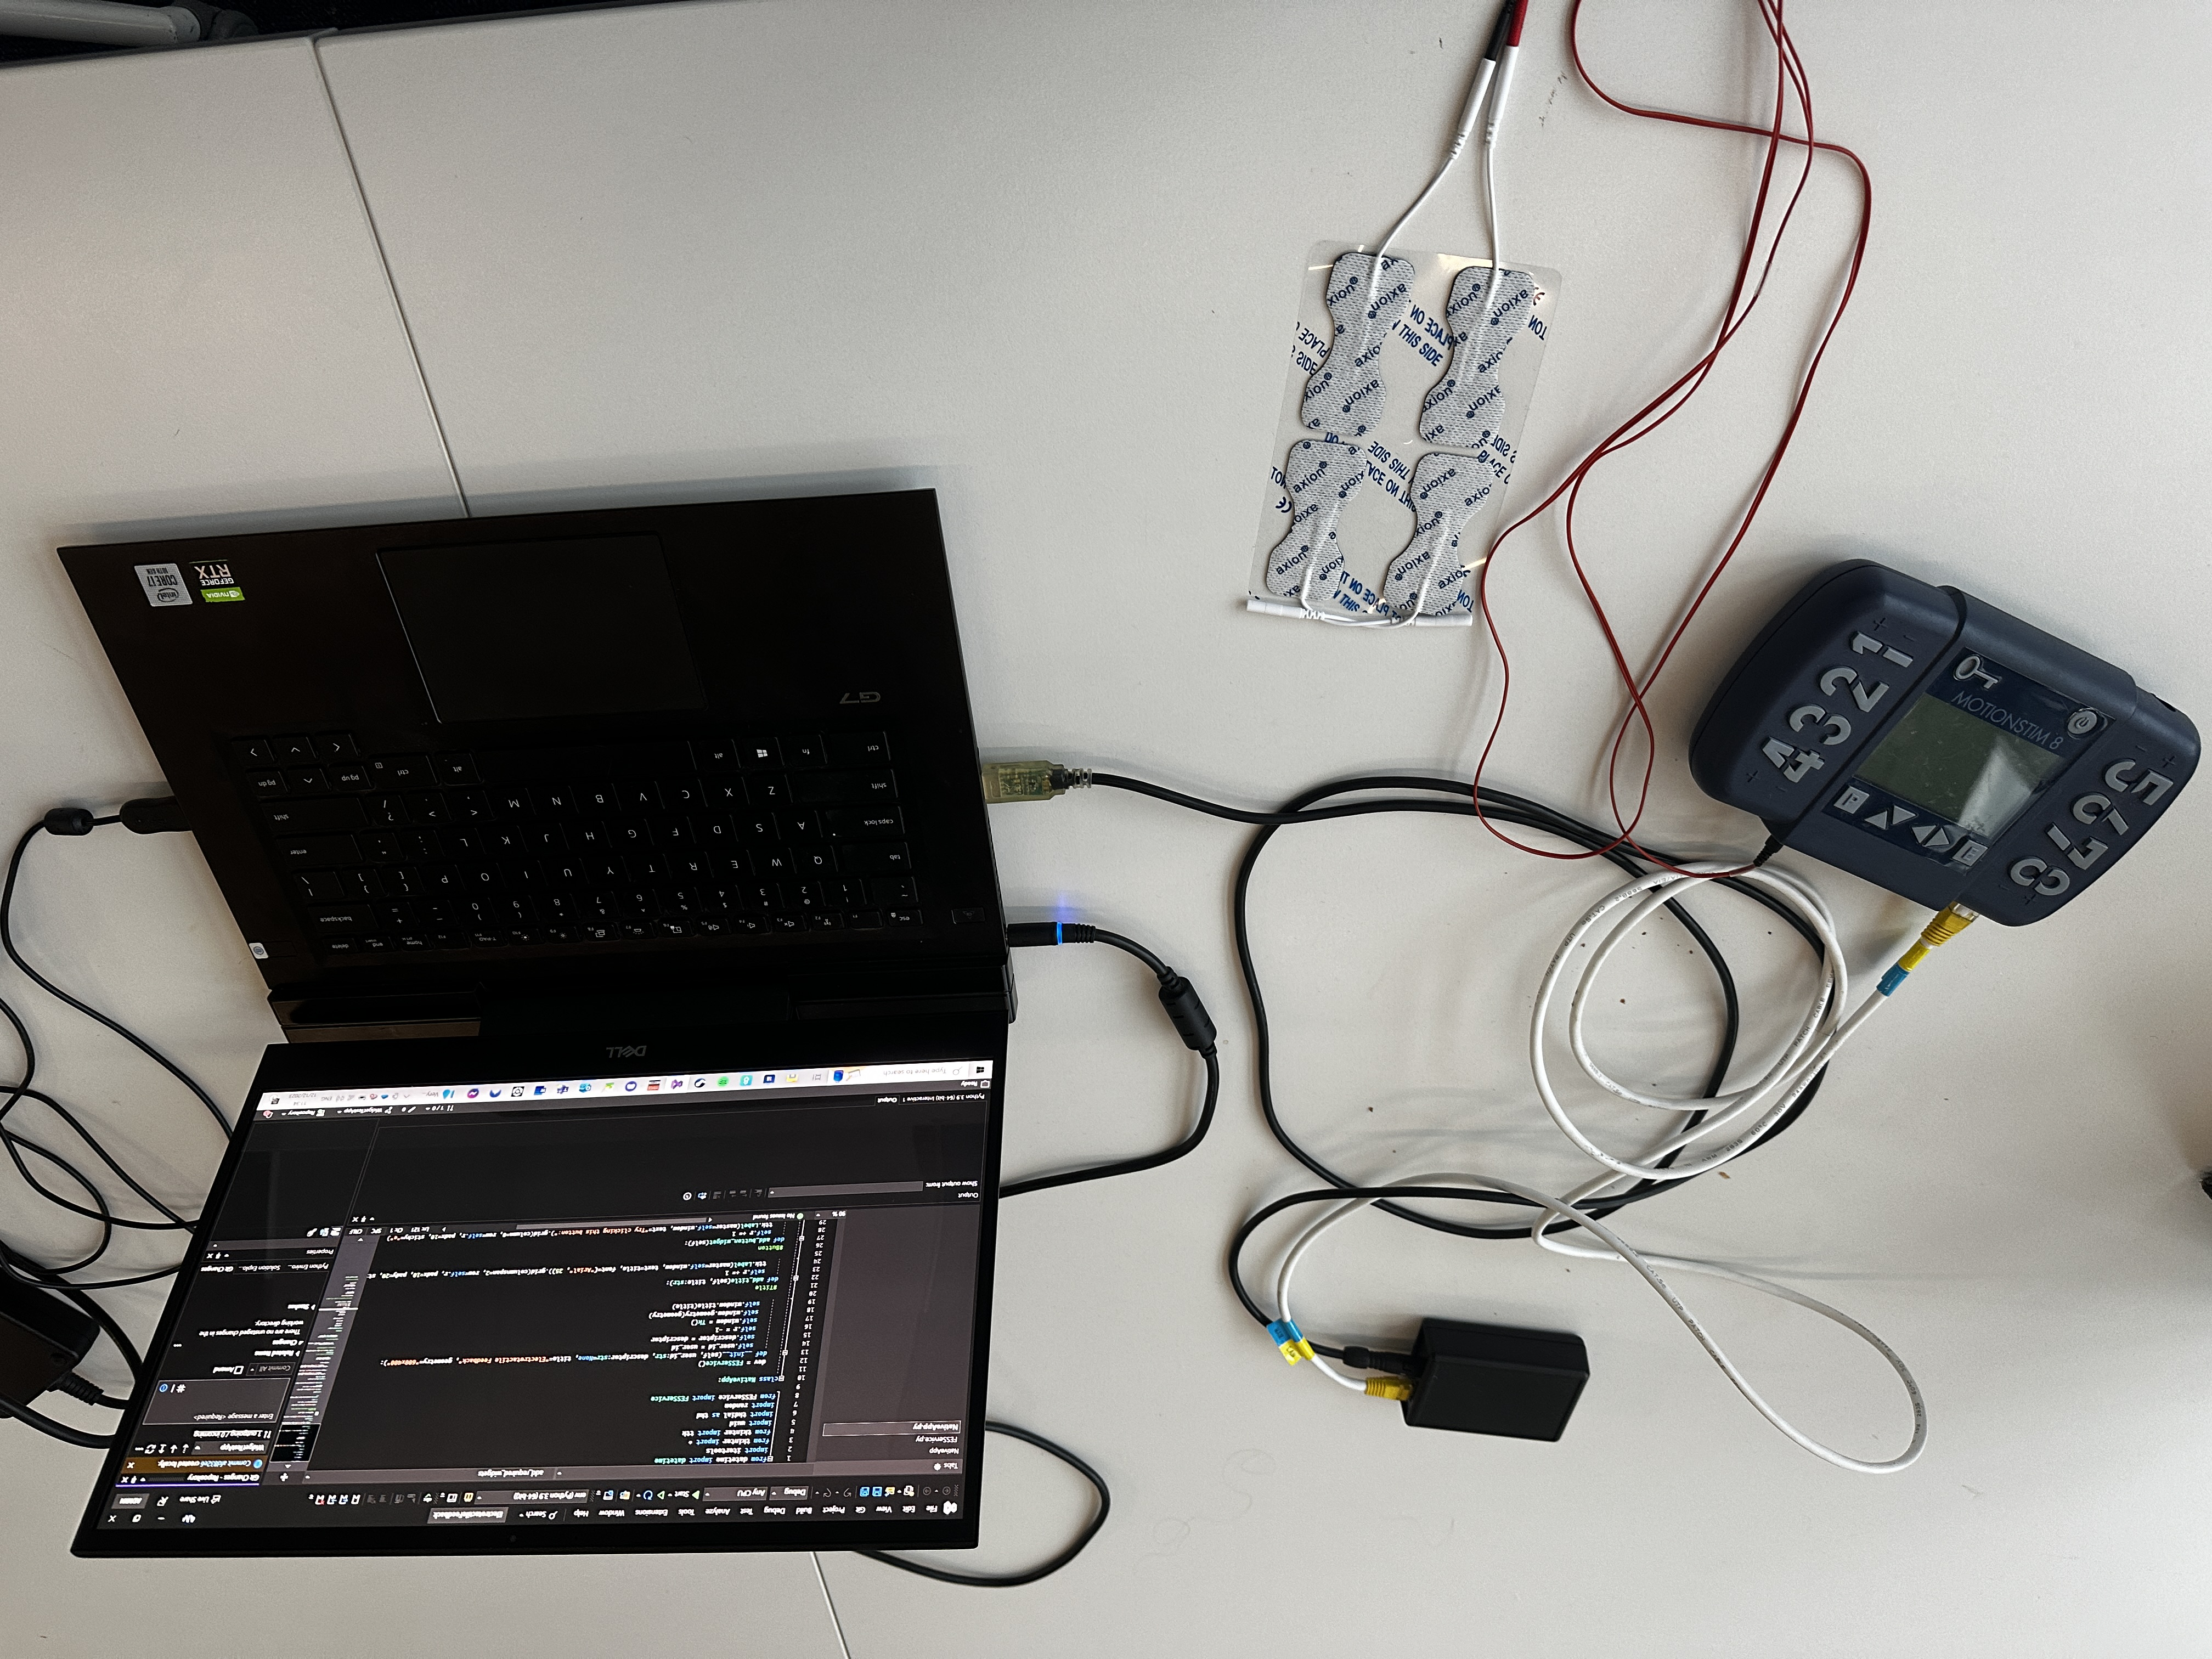
\includegraphics[scale=0.23, angle=180]{images/IMG_5137.JPG}
    \caption{Laptop with the application code open, the MOTIONSTIM 8 device on the left, connected to axion electrodes.}
    \label{fig:apparatus}
\end{figure}

\section{Evaluation One: Continuous Parameters} \label{sec:eval-1}
\subsection{Objectives and Hypotheses}
The primary objective of the first experiment was to ascertain the spectrum of electrotactile parameter settings which users perceive as appropriate. The settings under consideration include pulse-width, frequency, and amplitude. We were also interested to see how the various widget types compare to each other. As such, we sought to identify potential clusters in the data based on the type of interaction.

\subsection{Design, Setup and Procedure} \label{sec:design-1}
We decided that the best approach would be to present participants with four different widget types: a button widget; a selection of five radio button widgets; five multiple-select boxes; and finally, a text input widget. We would allow them to interact with these and tune each of the electrotactile parameters freely. They would do so until an appropriate signal was perceived from the interaction, then their chosen values would be recorded and the results grouped by widget type.

The application mentioned in section \ref{software-requirements} was configured such that it would present users with a window containing one of the four different widgets mentioned. The window also contained three dials and a save button. Each of the dials controlled the strength of a single electrotactile parameter. Limits were set for each parameter, to prevent major discomfort among users (pulse-width was limited to 200${\mu}s$, frequency to 100$PPS$ and amplitude was capped at 20$mA$). 

Two self-adhesive electrodes were attached to the palm of the participants' non-dominant hand, similar to that shown in Figure \ref{fig:hand}. Care was taken to ensure placement of the electrodes was kept as consistent as possible between participants. The anode (red) was placed at the top of their hand and the cathode (black) at the bottom. The gap between the electrodes was also taken into consideration - approximately 1cm, as far as was possible.

\begin{figure}
    \centering
    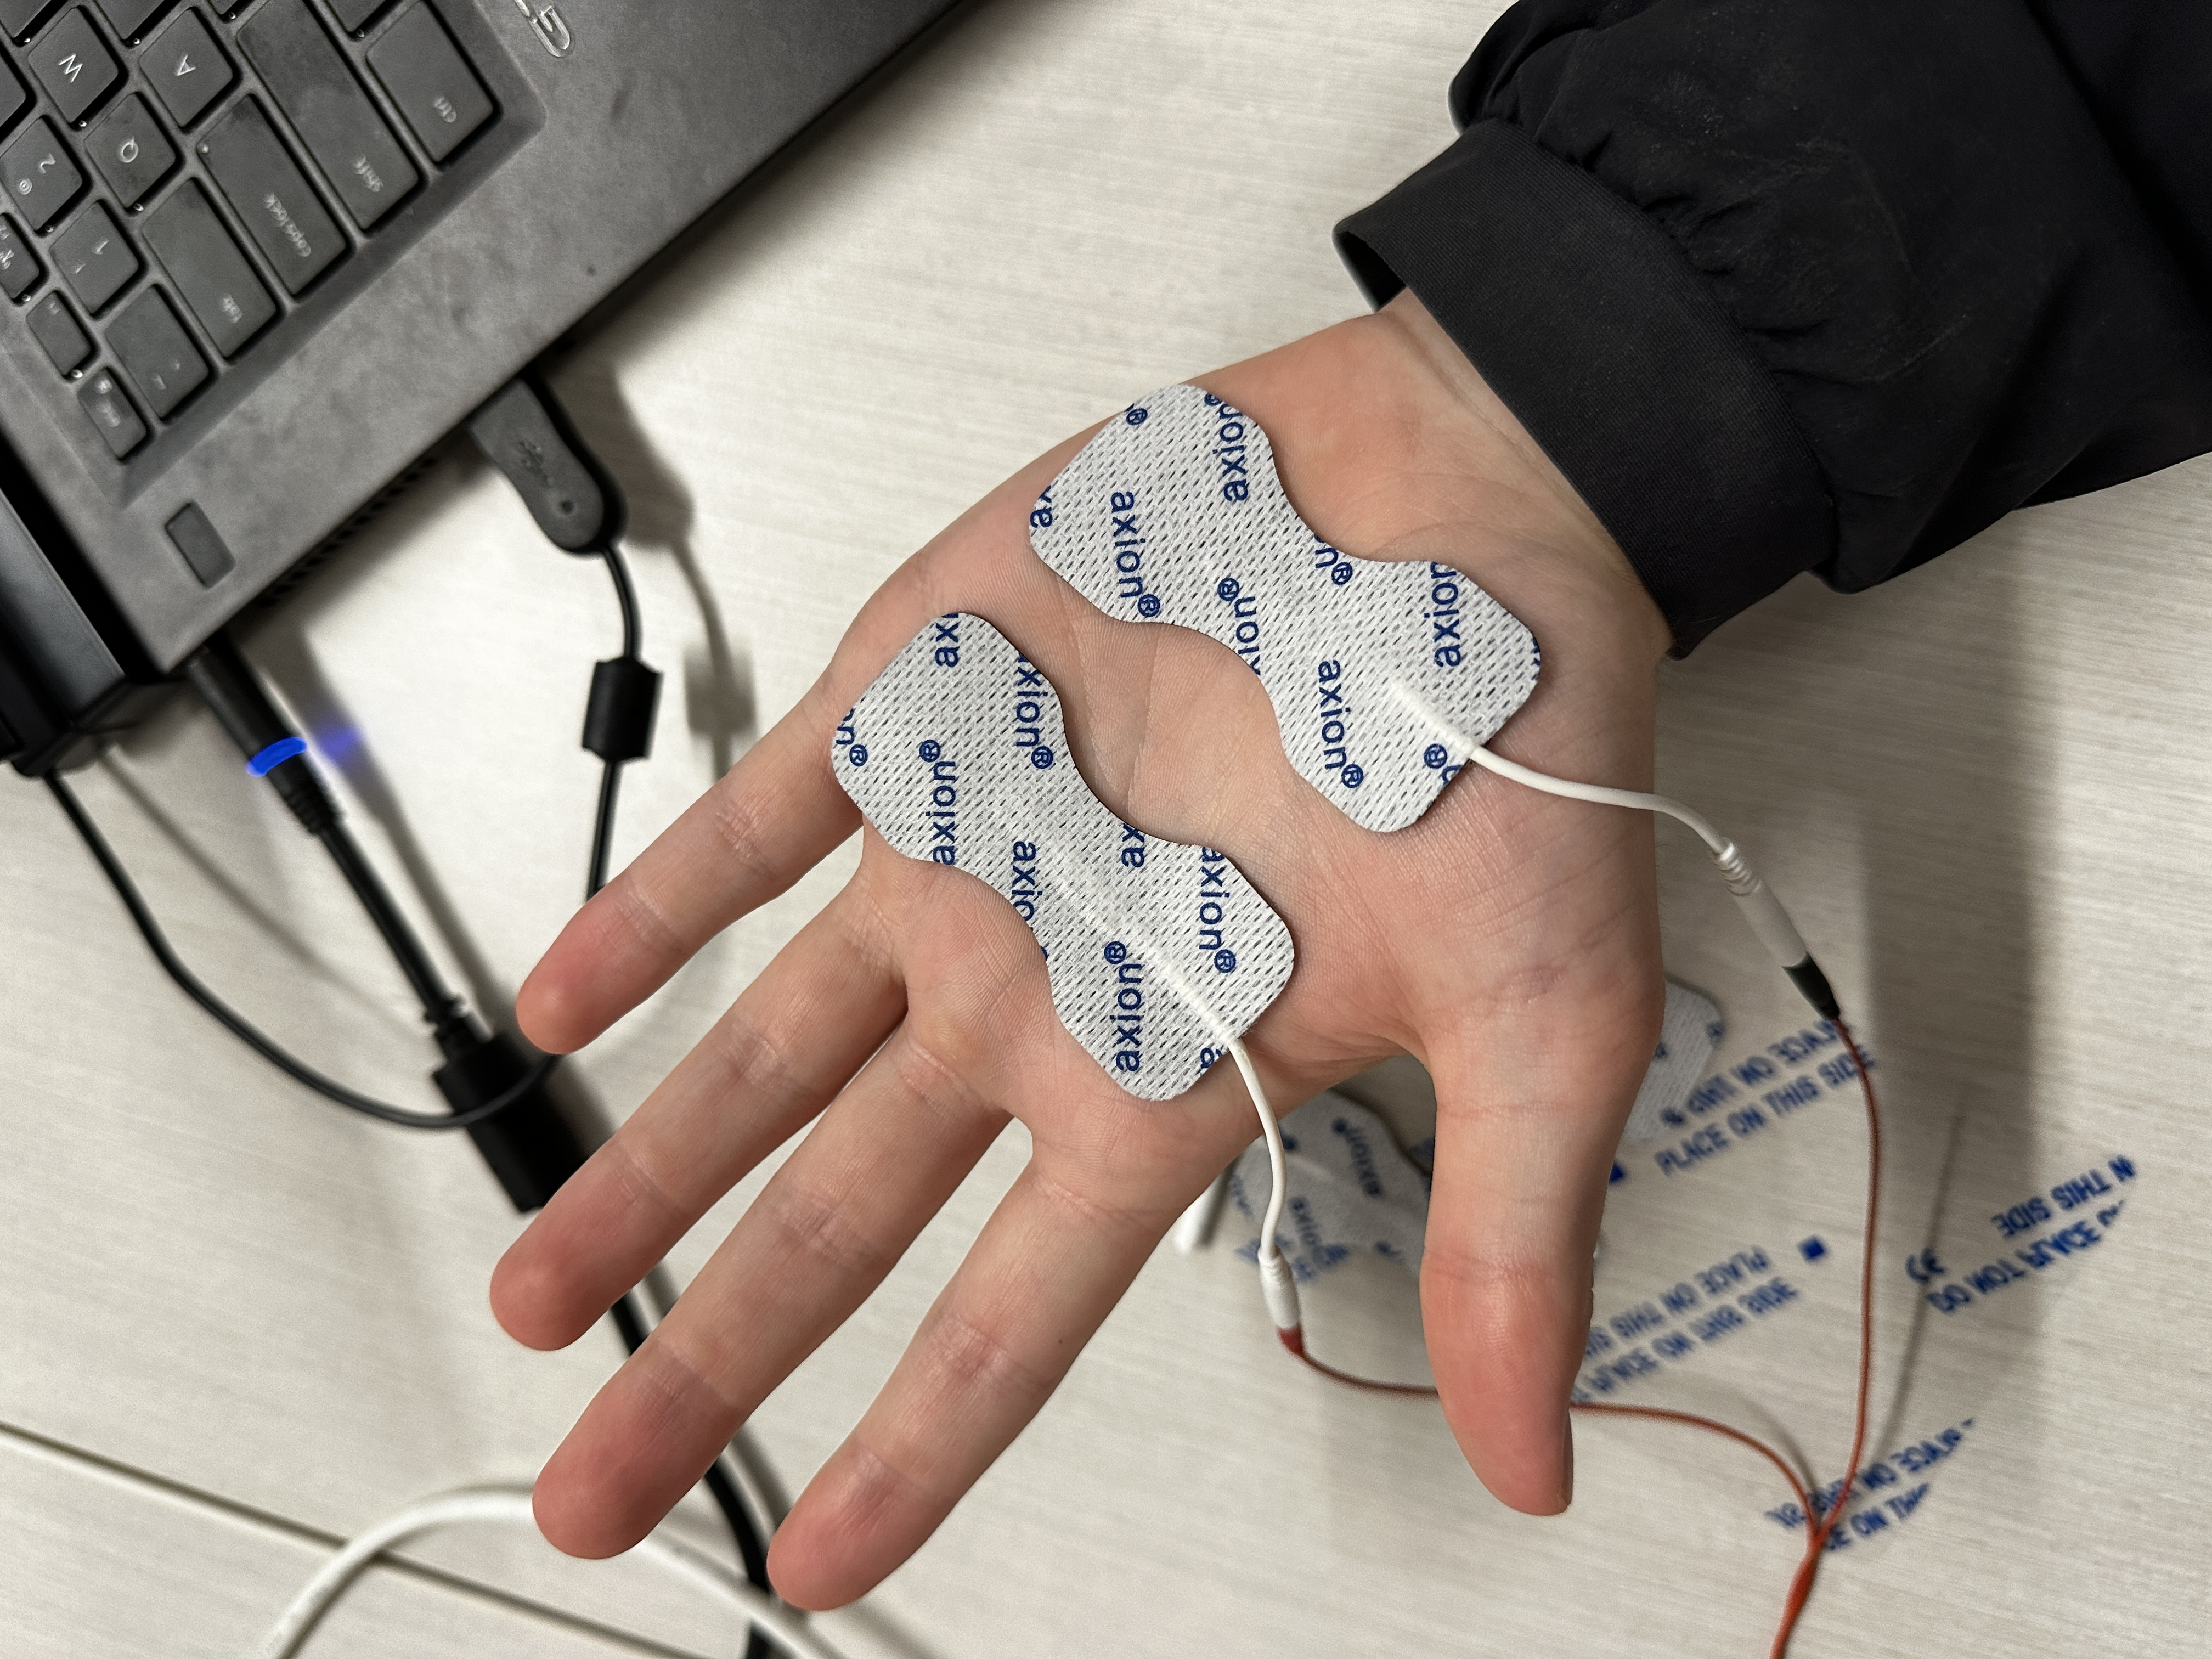
\includegraphics[scale=0.2, angle=270]{images/IMG_5135.JPG}
    \caption{A participant's hand connected to the FES device, using two self-adhesive electrodes.}
    \label{fig:hand}
\end{figure}

A demonstration window (which contained a button widget and where results were not recorded) was first shown to participants. This served two purposes. First, it aided in the explanation of what was required of the participants. Secondly, it allowed users to become familiar with the app and electrotactile sensation, without the pressure of their response being collected. Following this, each of the four widget types was presented to the participants, three times over. The order in which widgets were presented to users was random and parameter values were seeded from a different point on each occurrence of the same widget. This was to reduce the likelihood of participants selecting the same values each time, artificially. 

Participants were asked to interact with the widget displayed on the window. For the clickable widgets (all except the text input) the electrotactile signal was sent to the participant on a mouse-up event. Subjects were to tune each dial until the perceived cue was at an appropriate level for the widget in which they were interacting. After they were happy with their chosen values, subjects would hit the save button to record the results. This process was repeated until they had completed all 12 windows. Refer to Figure \ref{fig:tactile-application1} for an example button widget window shown to users.

\begin{figure}
    \centering
    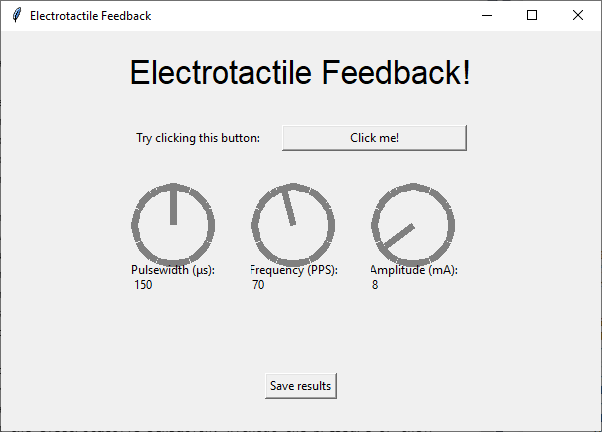
\includegraphics[scale=0.35]{images/tactile_application.png}
    \caption{Application GUI, set up for phase one, including button widget and dials to control signal strength.}
    \label{fig:tactile-application1}
\end{figure}

Upon completing the task described above, participants were asked to complete a short questionnaire. This was to collect some qualitative findings about their experience with electrotactile feedback. 

\subsubsection{Participants} \label{subsec:participants-1}
In total, 11 people participated in this evaluation (8 male and 3 female), recruited primarily through word of mouth, and social networks. Five participants were aged between 19 and 21, four were aged between 22 and 25, with only two participants being older than this - one aged between 26 and 30, the other being 40+. All participants were right-handed, so electrodes were placed on their left hands. We excluded participants who were pregnant, or who had any underlying heart conditions.

\subsection{Results} \label{results-1}
After experimentation had concluded, results were collated and processed. During this process, 3D scatter plots were conceived - showing pulse-width on one axis, frequency on the second, and amplitude on the third. Metrics such as means and standard deviations were calculated for different groupings.

The first of the 3D charts simply plotted every response on the same chart (12 responses per user). This was primarily to see if, at a high level, there were any obvious clusters or trends. Perhaps unsurprisingly, this did not yield much meaningful data. The means and standard deviations were, nevertheless, calculated here to be as follows: pulse-width was found to be approximately $96.5{\mu}s$ ($SD\approx35.63{\mu}s$); the frequency was near $52.4 PPS$ ($SD\approx22.8PPS$); and the amplitude, roughly $11.04mA$ (with $SD\approx2.94mA$).

Next, responses were grouped by widget type and four charts were produced. These plots can be seen in Figure \ref{fig:widget-clusters} and contain each of the three responses made by subjects, per widget. While the results here still displayed a high level of standard deviation, the data was more meaningful than the first chart and would go on to form the basis of the subsequent evaluation (see Section \ref{sec:design-2}). Once again, the means and standard deviations were calculated - the values of which can be seen in Table \ref{tab:widget-means}.

\begin{figure}
    \centering
    \begin{subfigure}{0.22\textwidth}
        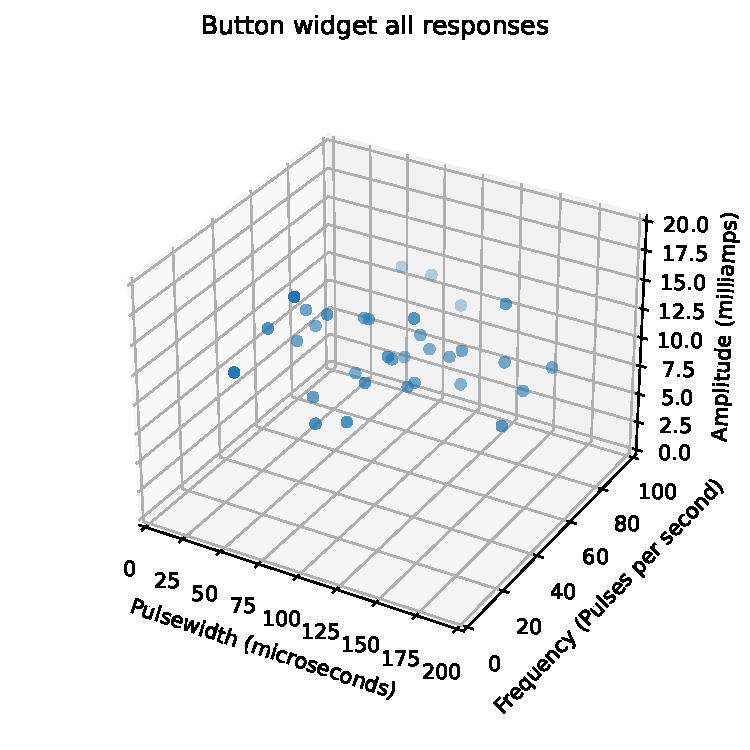
\includegraphics[width=\textwidth]{images/20240321-134009.pdf}
    \end{subfigure} \hfill
    \begin{subfigure}{0.22\textwidth}
        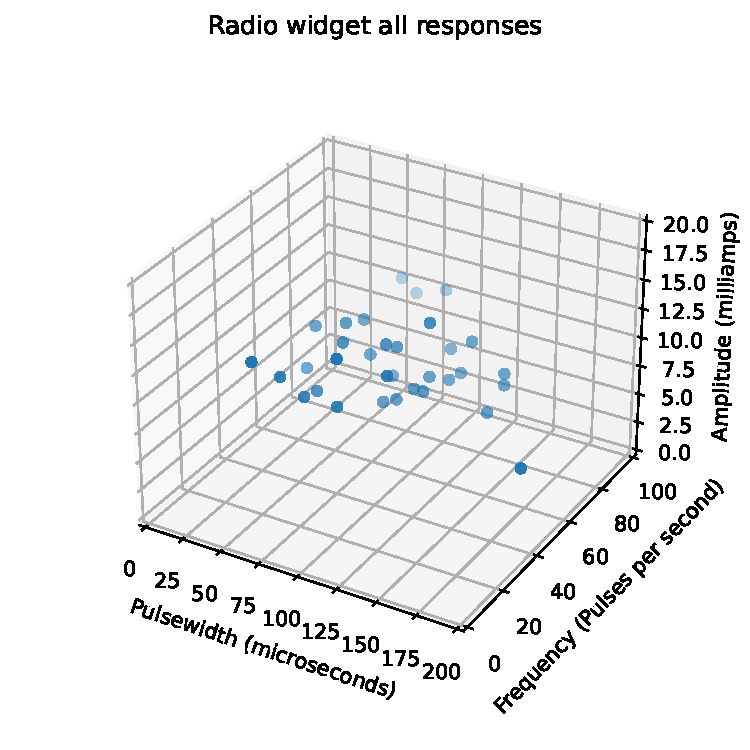
\includegraphics[width=\textwidth]{images/20240321-134107.pdf}
    \end{subfigure} \hfill
    \begin{subfigure}{0.22\textwidth}
        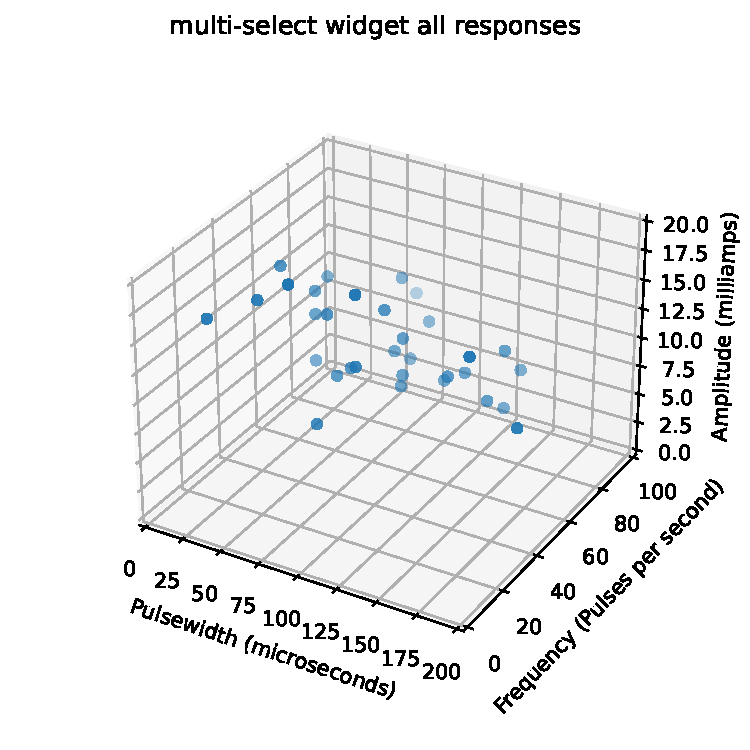
\includegraphics[width=\textwidth]{images/20240321-134134.pdf}
    \end{subfigure} \hfill
    \begin{subfigure}{0.22\textwidth}
        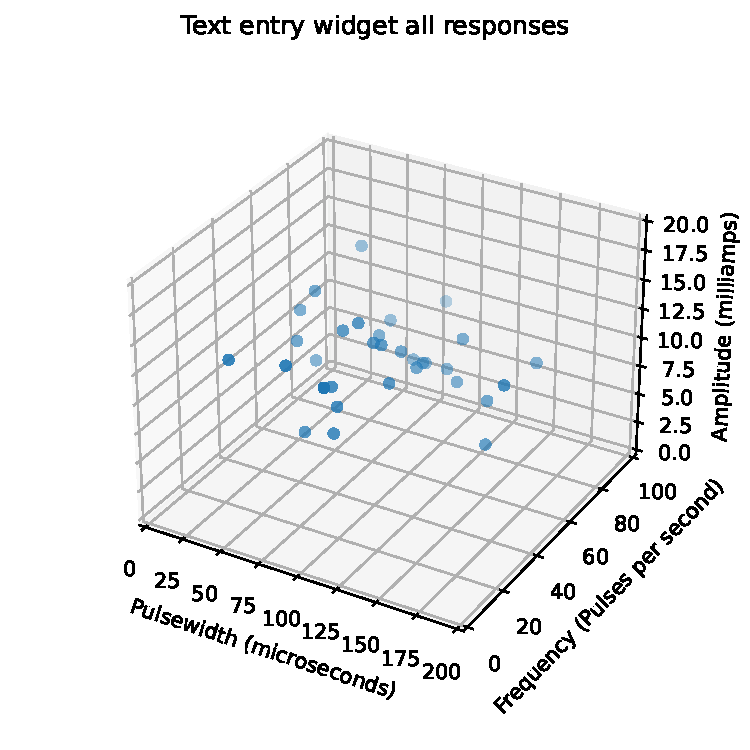
\includegraphics[width=\textwidth]{images/20240321-134214.pdf}
    \end{subfigure} \hfill
    \caption{Charts showing every combination of parameters for each of the four widget types.}
    \label{fig:widget-clusters}
\end{figure}

\begin{table}
\resizebox{\columnwidth}{!}{
\begin{tabular}{ll|l|l}
\multicolumn{2}{c|}{Widget Style} & \multicolumn{1}{c|}{Mean}  & \multicolumn{1}{c}{Standard Deviation} \\ \hline
\multicolumn{1}{l|}{\multirow{3}{*}{Button}}       & Pulse-Width (${\mu}s$)  & 97.1  & 34.9       \\
\multicolumn{1}{l|}{}                              & Frequency (PPS) & 53.9  & 22.9               \\
\multicolumn{1}{l|}{}                              & Amplitude (mA)  & 11.2  & 2.82               \\ \hline
\multicolumn{1}{l|}{\multirow{3}{*}{Radio}}        & Pulse-Width (${\mu}s$)  & 100.0 & 33.4       \\
\multicolumn{1}{l|}{}                              & Frequency (PPS) & 51.8  & 22.7               \\
\multicolumn{1}{l|}{}                              & Amplitude (mA)  & 10.5  & 2.28               \\ \hline
\multicolumn{1}{l|}{\multirow{3}{*}{Multi-Select}} & Pulse-Width (${\mu}s$)  & 92.5  & 40.4       \\
\multicolumn{1}{l|}{}                              & Frequency (PPS) & 53.7  & 22.3               \\
\multicolumn{1}{l|}{}                              & Amplitude (mA)  & 11.7  & 3.65               \\ \hline
\multicolumn{1}{l|}{\multirow{3}{*}{Text}}         & Pulse-Width (${\mu}s$)  & 96.6  & 33.0       \\
\multicolumn{1}{l|}{}                              & Frequency (PPS) & 50.3  & 21.1               \\
\multicolumn{1}{l|}{}                              & Amplitude (mA)  & 10.8  & 2.68              
\end{tabular}
}
\caption{\label{tab:widget-means} Means and standard deviations obtained from grouping results by widget type.}
\end{table}

\begin{figure}
    \centering
    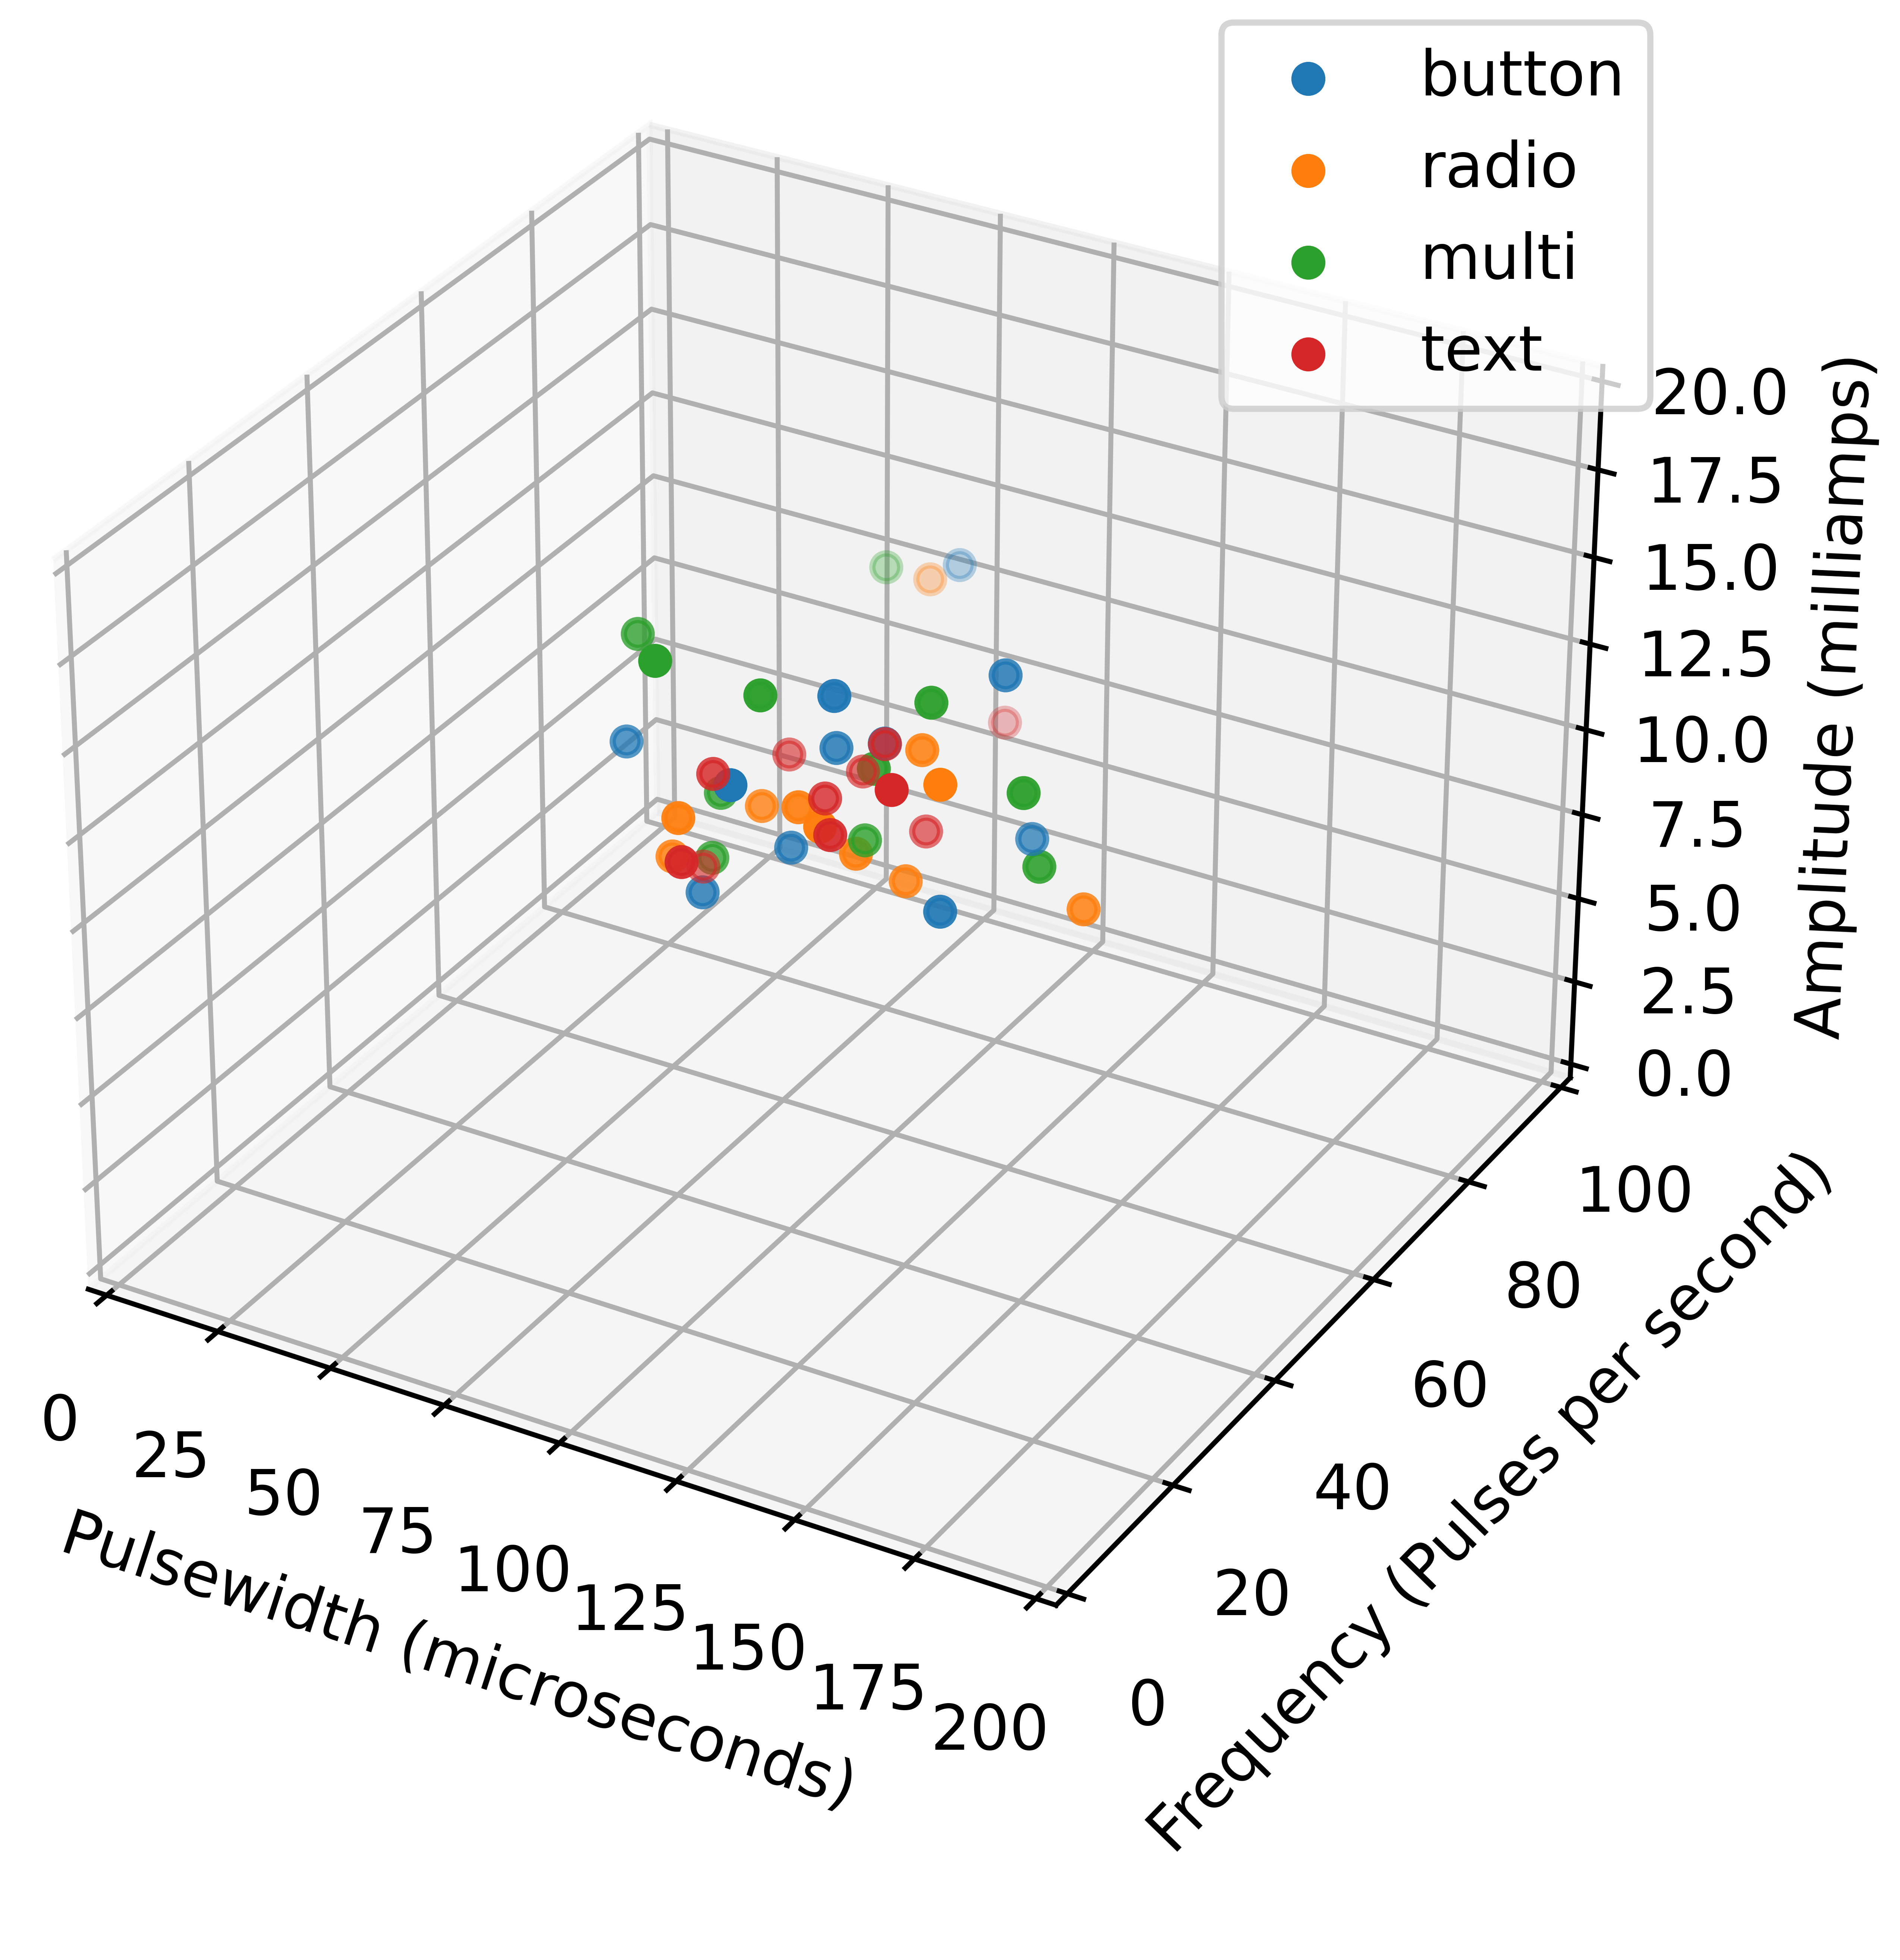
\includegraphics[scale=0.5]{images/avg_responses_widgets.png}
    \caption{Average user values across each response for each widget}
    \label{fig:avg-user-responses-widgets}
\end{figure}

Following this, two additional charts were plotted. One of these contained points representing the average values of each user, over every response. The other was similar but instead plotted four points per user - each representing an average of the three responses for each widget type. This chart can be viewed in Figure \ref{fig:avg-user-responses-widgets}.

Other charts and metrics were computed, including charts showing how individuals responded. These graphs, along with interactive versions of all others mentioned here are available to view from the first ipynb file provided on GitHub.\footnote{\url{https://github.com/AaronMilne19/electrotactile-feedback/blob/525683bfec8519a3c0c7227c2b925527da2b54a0/data/notebooks/electrotactile_results_analysis.ipynb}}\\

\subsection{Discussion} \label{discussion-1}
Upon examination of the results, particularly the depiction shown in Figure \ref{fig:avg-user-responses-widgets}, it is evident that 
the four distinct clusters corresponding to widget style, which we had anticipated, were not identified. This thought was amplified by the high values of standard deviation obtained across responses, suggesting a wide range of values being selected among users. This was interesting, nevertheless, as it highlighted the subjective nature of electrotactile cues, indicating the difficulty in finding a suitable strength for all. This could be due to variability in user tolerance to signals, potential desensitisation as subjects progress through the evaluation, and individual opinions of electrotactile feedback in general.

While there was no evidence of distinct clusters appearing for different widgets, an overall cluster emerged when we looked more generally across every widget. Concerning Figure \ref{fig:avg-user-responses-widgets}, approximately 69\% of points fell within the following range: pulse-width values between $60{\mu}s$ and $130{\mu}s$; frequency values between 30PPS and 65PPS; and amplitude values between 9 and 15 milliamps. This forms the boundary for an optimal cluster which we will discuss further.

This finding is intriguing since it suggests there is no correlation between different widget types and a user's preference for electrotactile strength. Moreover, it does propose the theory of an optimal zone for signal strength. Based on this theory, ideal settings for electrotactile signals will likely lie somewhere in this domain. The second evaluation (Section \ref{eval2}) aims to explore this theory further.\\ 

\subsubsection{Limitations}
A possible reason behind the lack of evidence appearing for widget-based clusters could have been due to uncertainty in our data. A source of this includes the number of participants recruited to take part, which was sub-optimal. As mentioned in Section \ref{subsec:participants-1}, we managed to recruit only 11 participants. While this number gave us sufficient results, the data obtained would have been much more robust, given an increase in subject numbers. 

Factors behind the low sign-up rate include the timing of the experiment. It was performed during the final week of the first semester and the subjects were primarily students, a lot of whom are commonly unavailable during this time. Furthermore, no incentives could be offered for recruitment. This would have boosted turnout.

\subsubsection{Questionnaire}\label{subsubsec:questionnaire-1}
The questionnaire shown to participants at the end of the experiment, allowed us to collect some qualitative data about their thoughts on electrotactile feedback. Due to the similarity in nature, the responses were combined with those obtained from the second evaluation. Refer to section \ref{subsec:questionnaire-1-2} for analysis of the responses to both questionnaires.

\section{Evaluation Two: Discrete Presets} \label{eval2}
\subsection{Objectives and Hypotheses}
Following the outcomes of the first evaluation, we decided that the second study should focus on further exploring the optimal region outlined in Section \ref{discussion-1}. During this process, we would also look for preset(s) that satisfy the preferences of users across the board.

\subsection{Design, Setup and Procedure} \label{sec:design-2}
The approach taken for this evaluation closely resembled that of the previous (Section \ref{sec:design-1}). The same apparatus was used (Figure \ref{fig:apparatus}) and the experiment was orchestrated consistently. The two self-adhesive electrodes were positioned, as before, on the palms of participants' non-dominant hands, in as harmonious a way as possible to Figure \ref{fig:hand}. Again, users undertook a similar task of interacting with the same four widget types as before (button, radio, multiple-select and text), three times each. They would again experience electrotactile feedback as they interact with these widgets.

The key difference between this study and the last was that previously, subjects were to choose parameters from a continuous range of values. This time, participants were asked to attempt five discrete presets before deciding on their favourite. Users were also advised, on the final window, to decide an order of preference for presets from best to worst. Furthermore, they were asked, at this time, to note any presets that they could not perceive due to the setting being too weak. 

The application was altered slightly to suit these requirements. Five radio buttons were added to the user interface, in place of the dials from the previous evaluation. These were labelled 'Preset 1' through 'Preset 5'. You can see how this appeared to users, by referring to Figure \ref{fig:tactile-application2}. Some additional alterations were also made to the app at a lower level during this time - for instance, how the preset buttons on the user interface physically affected the signal strength sent through the device. 

After the initial demonstration window, the order of presets was randomised. This was to reduce the predictability of electrotactile signals and to prevent users from intentionally selecting the same presets each time. Furthermore, a mechanism was added to prevent users from saving results without having first attempted all presets. This acted as a safety guard, preventing participants from submitting before intended. 

\begin{figure}
    \centering
    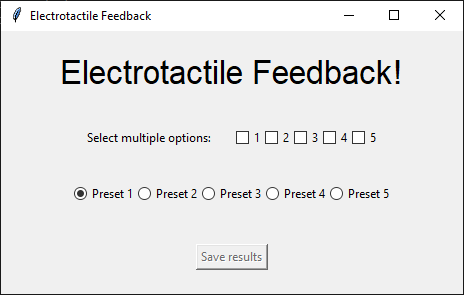
\includegraphics[scale=0.5]{images/Screenshot 2024-02-24 151633.png}
    \caption{Application GUI, set up for phase two. Contains our multiple-selection widget for interaction and radio buttons, indicating presets of varying strength.}
    \label{fig:tactile-application2}
\end{figure}

\begin{table*}
\centering
\begin{tabular}{c|ccc|ccc|ccc|ccc|ccc}
\multirow{2}{*}{Preset} & \multicolumn{3}{c|}{1} & \multicolumn{3}{c|}{2} & \multicolumn{3}{c|}{3} & \multicolumn{3}{c|}{4} & \multicolumn{3}{c}{5} \\ \cline{2-16} 
                        & PW    & FQ    & AMP    & PW    & FQ    & AMP    & PW    & FQ    & AMP    & PW     & FQ    & AMP   & PW     & FQ   & AMP   \\ \hline
Button                  & 64    & 29    & 8      & 78    & 42    & 10     & 92    & 56    & 11     & 116    & 70    & 12    & 139    & 85   & 14    \\
Radio                   & 66    & 20    & 8      & 81    & 34    & 9      & 97    & 47    & 10     & 115    & 56    & 12    & 132    & 66   & 13    \\
Multi                   & 50    & 23    & 8      & 70    & 36    & 10     & 89    & 49    & 11     & 113    & 59    & 14    & 137    & 70   & 16    \\
Text                    & 59    & 20    & 8      & 78    & 34    & 9      & 97    & 49    & 11     & 118    & 59    & 12    & 139    & 70   & 14   
\end{tabular}
\caption{\label{tab:presets}Final preset values used for the second evaluation.}
\end{table*}

Another alteration was made, such that instead of users receiving just one electrotactile cue (on a mouse-up event), they would now receive one on both mouse-down and mouse-up events. We considered the advantages and disadvantages of making this amendment. This would change the user experience slightly from the first study, a decision which could have impacted the results obtained, had it been in place during the first evaluation. Conversely, the feedback experienced would provide users with a more realistic sensation than before. We, therefore, decided to move forward with this approach, despite the minor change to consistency.

Once again, a questionnaire was posed to participants upon completion of the experiment. This questionnaire was designed to gather similar information to that of the first study. As a result, several questions were identical. This allowed us to combine responses to these questions, from both questionnaires to produce a more robust analysis.

\subsubsection{Participants}\label{subsec:participants-2}
We managed to recruit 12 participants to take part in this evaluation (2 female and 10 male). Word of mouth and social networks was once again the primary method of recruitment. For this evaluation, we chose to exclude not only people who were pregnant, or who had any underlying heart conditions. But also those who took part in the first evaluation - as these people would not be naive subjects. Of the recruited participants, six were aged between 19-21 and six were aged between 22-25. Once again, all participants were right-handed so the electrodes were positioned on the palm of their left hands.

\subsection{Determining Presets}

The next challenge was to determine the values that each of the five presets should carry - a deterministic approach to choosing these was essential. There were several metrics to look at from the first evaluation (Section \ref{results-1}), however, we decided on an approach which made use of the mean values for each widget. 

This approach first entailed the removal of any points which lay further than two standard deviations from the mean responses of study one (Section \ref{results-1}). This prevented any outliers in results affecting the final preset values. After the pulse-widths, frequencies and amplitudes had all been truncated, the mean values of the remaining responses formed the median strength preset (preset 3). This process was repeated four times, once for each widget type. It should be noted that the values used for this preset differ from the mean values shown in table \ref{tab:widget-means}. This is due to the removal of values during truncation.


\begin{figure}
    \centering
    \includegraphics[scale=0.017]{images/Merged_document.png}
    \caption{Bar charts for each of the four widget types: button, multi-select, radio and text (top left to bottom right). Charts display presets one through five - in ascending order of strength - against the number of times it was chosen by subjects. }
    \label{fig:preset-results}
\end{figure}

\begin{table}
\resizebox{\columnwidth}{!}{
\begin{tabular}{l|lllll}
\textbf{User} & \textbf{Best} & \textbf{Second Best} & \textbf{Third Best} & \textbf{Second Worst} & \textbf{Worst} \\ \hline
1             & 3             & 2                    & 4                   & 5                     &                \\
2             & 2             & 3                    & 4                   & 5                     &                \\
3             & 3             & 2                    & 4                   & 5                     &                \\
4             & 4             & 3                    & 5                   & 2                     &                \\
5             & 2             & 3                    & 1                   & 4                     & 5              \\
6             & 3             & 2                    & 4                   & 5                     &                \\
7             & 5             & 4                    &                     &                       &                \\
8             & 3             & 4                    & 5                   &                       &                \\
9             & 4             & 3                    & 5                   &                       &                \\
10            & 3             & 2                    & 4                   & 5                     &                \\
11            & 3             & 2                    & 4                   & 5                     &                \\
12            & 4             & 3                    & 5                   &                       &               
\end{tabular}
}
\caption{\label{tab:user-preferences}User preferences of presets (for button widget) from best to worst. Presets increase from weakest to strongest.}
\end{table}

\begin{figure}
    \centering
    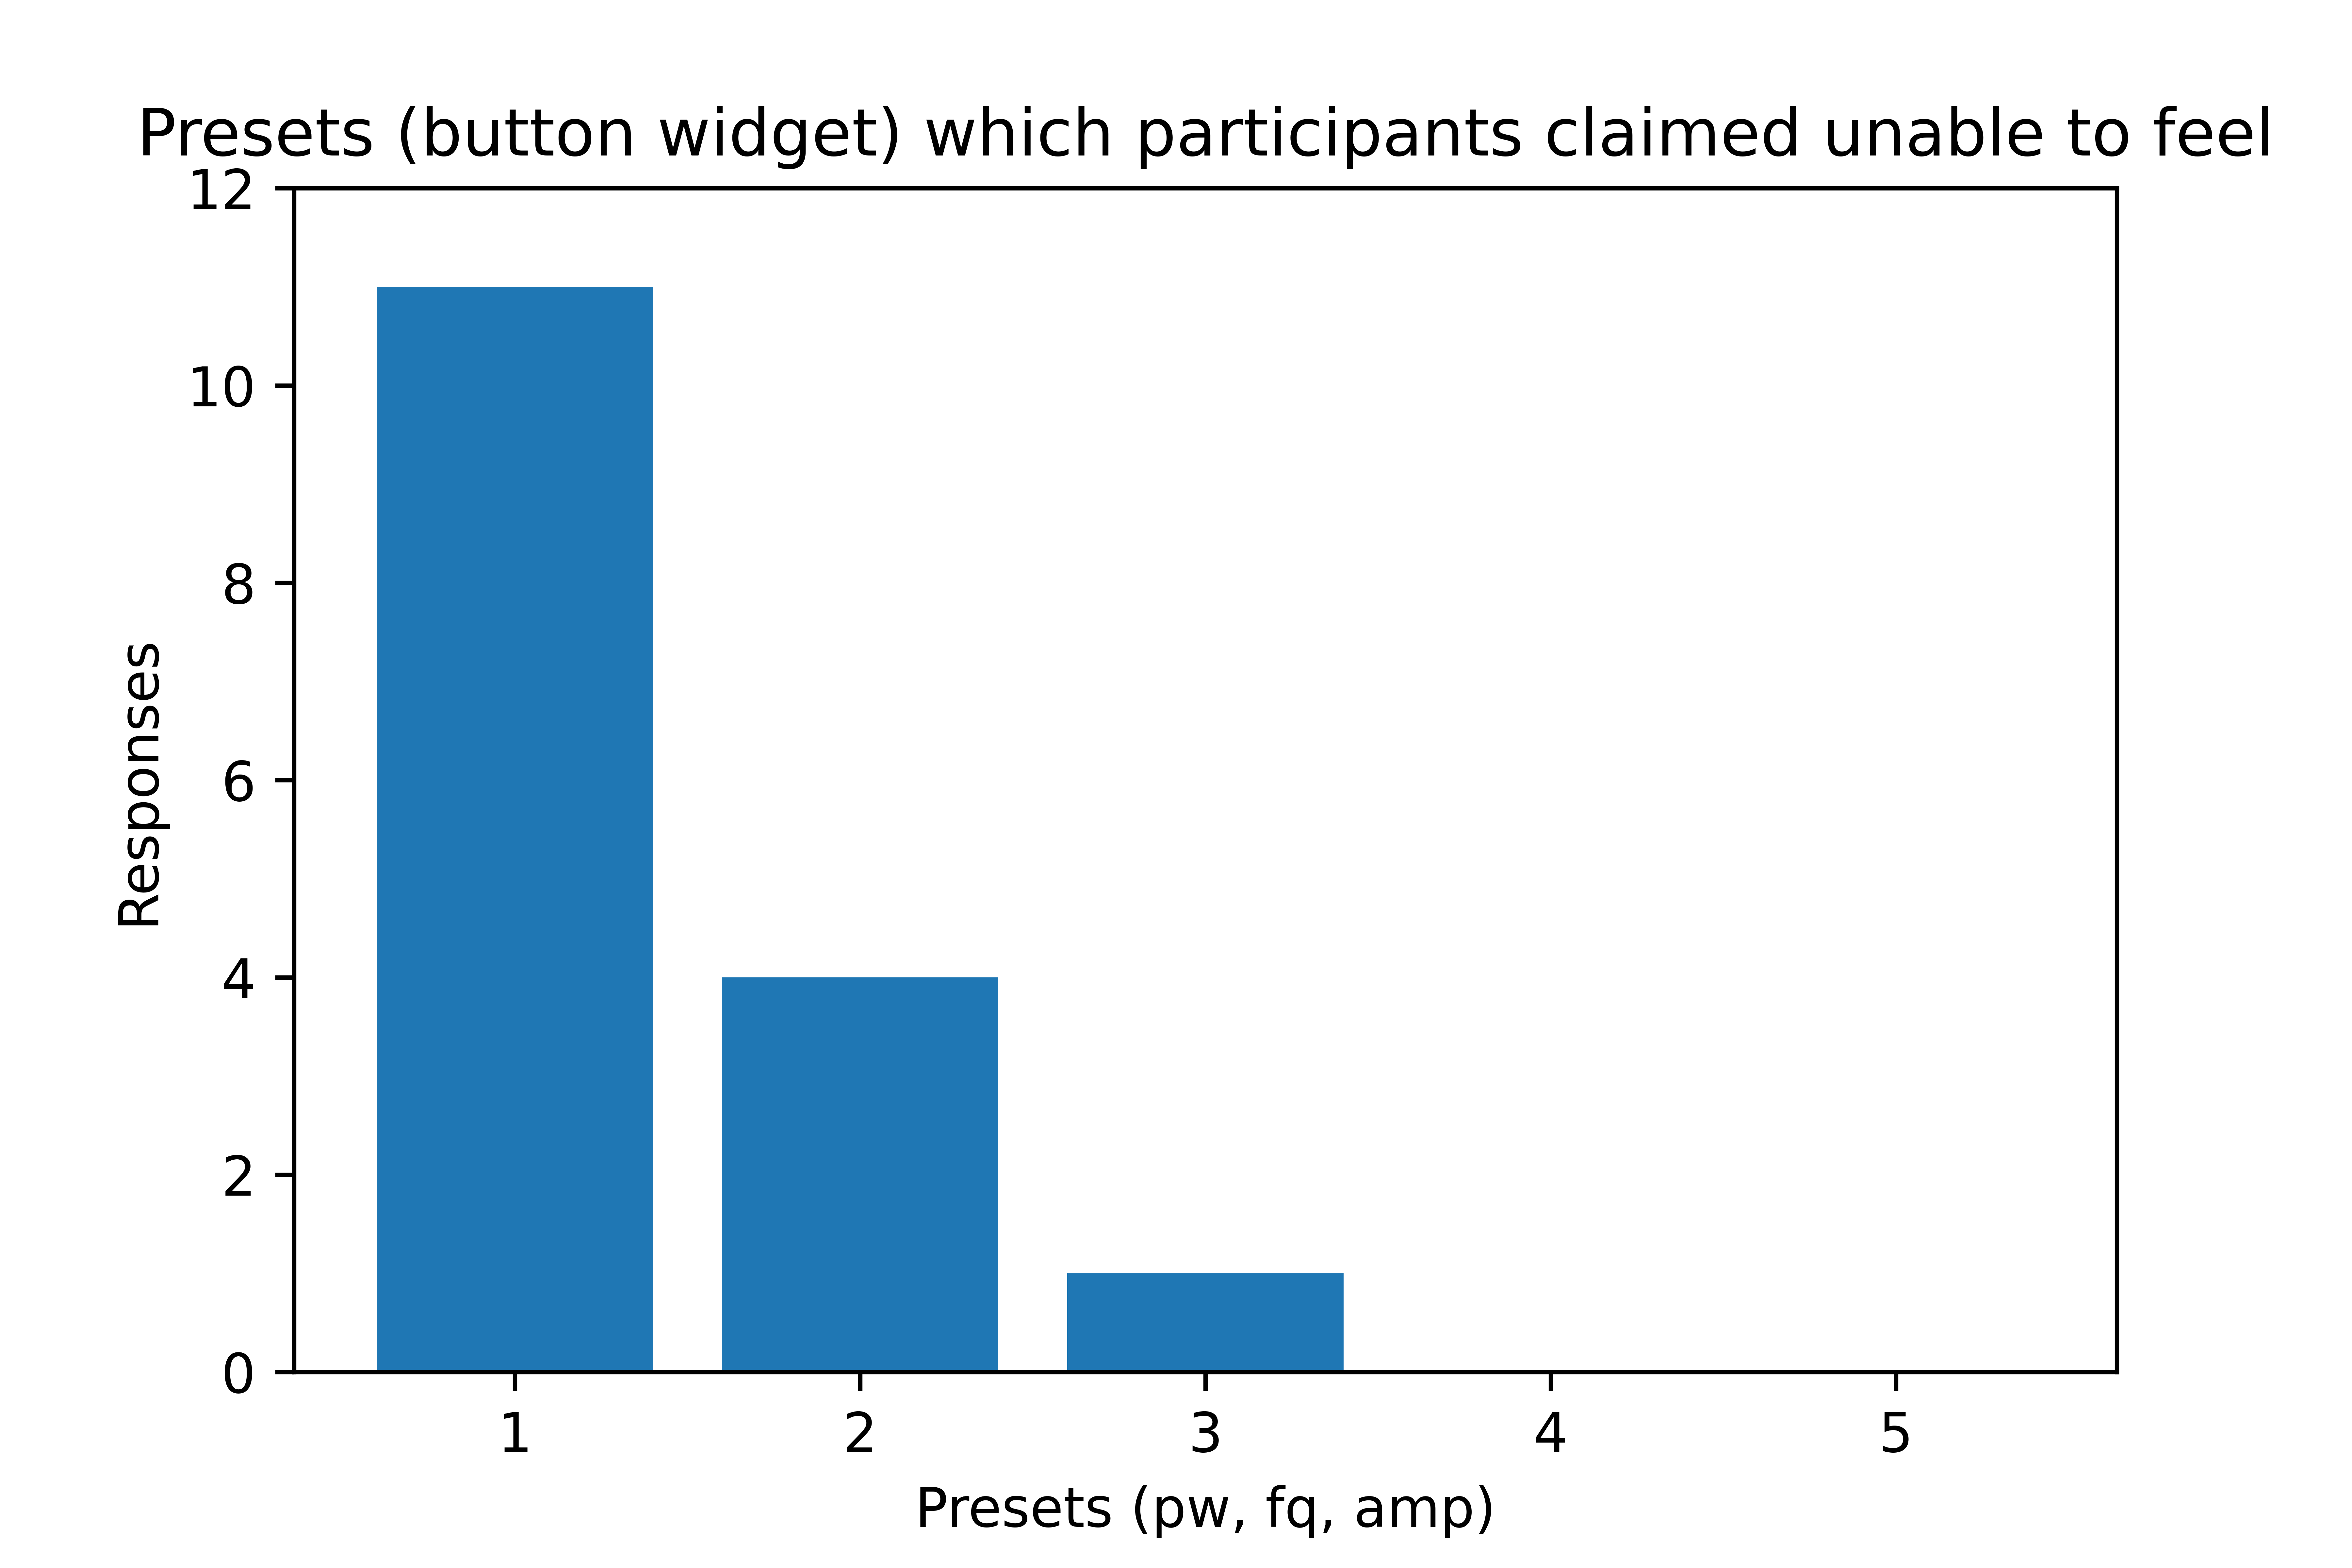
\includegraphics[scale=0.44]{images/Presets (button widget) which participants claimed unable to feel.png}
    \caption{Bar chart showing the number of participants that could not perceive certain presets (button widget).}
    \label{fig:presets-not-felt}
\end{figure}

Four additional presets were chosen, two carrying greater intensity than preset 3 and two with lesser. These were found by first, calculating step values for parameter values lying below (L) and above (R) the mean. stepL=(mean$-$ smallestVal)$\div$3 and stepR=(largestVal$-$mean)$\div$3. The two larger presets were then found by calculating mean$+$stepR and mean$+$(2$\times$stepR) across the three parameters. The two smaller presets were calculated similarly, by taking the mean value minus stepL and 2$\times$stepL respectively.

This process was undertaken for the four widgets and the final results are shown in Table \ref{tab:presets}. These represent the presets used during this study.\\

\subsection{Results} \label{results-2}
Results were again collated and processed after experimentation concluded. This time, bar charts were generated. We began by creating bar charts for each widget type, showing the preset value against the number of times it was selected by participants. These four charts are shown in Figure \ref{fig:preset-results}.

The charts of Figure \ref{fig:preset-results} show that for all four widgets, preset 3 was the favourite among users. It was chosen between 16 and 20 times per widget, out of a total of 36 responses (12 participants, 3 occurrences each). This equates to between 44.4\% and 55.6\% of responses, depending on the widget type being used. Preset 4 was a consistent second favourite, with it being chosen 19.4\% to 33.3\% of the time - widget-dependent - and preset 2 in third place, being chosen up to 16.67\% of times. Presets 1 and 5 were chosen with the least frequency, the first being picked a maximum of only two times (5.56\%), during text input widgets.

One additional window, containing a button widget was presented at the end of the experiment. The preset that users chose as their favourite was not recorded here. Instead, they were to decide on an order of preference for all five, ranking from best to worst. They were asked not to rank any presets that they could not perceive, but to instead note these separately. Table \ref{tab:user-preferences} shows the rankings chosen by users and Figure \ref{fig:presets-not-felt} shows presets against the number of times they went unperceived.

Several additional charts were plotted, including those showing how individual users responded, designed to compare users to themselves. These charts, as well as all others mentioned, are available on the second ipynb file on GitHub.\footnote{\url{https://github.com/AaronMilne19/electrotactile-feedback/blob/525683bfec8519a3c0c7227c2b925527da2b54a0/data/notebooks/electrotactile_results_phase2_analysis.ipynb}}\\

\subsection{Discussion}
As demonstrated in the previous section (\ref{results-2}), the median strength preset, preset 3, was found to be most popular among participants - with this being chosen 44.4\% to 55.6\% of the time (see Figure \ref{fig:preset-results}). This result is promising and satisfies our hypothesis. Given preset 3 was selected deterministically using the mean values achieved from our first evaluation, it fits almost perfectly centred within the cluster we observed before (with minor variances between widgets). The fact that this preset was found to be most favourable, reinforces our optimal window hypothesis.

The results of Table \ref{tab:user-preferences} reinforce the superiority of the median preset, as we can see that 50\% of participants noted this as the 'best' option. This closely aligns with the 52.8\% of button responses during the experiment, being for this preset. Moreover, five of the remaining six participants noted it as the 'second best' option, with the only exception claiming they were unable to perceive this preset.

As we moved further from the centre of the cluster, the less popular the presets became. This was shown via the fourth preset of each widget, which lay close to the upper boundary of the mentioned cluster. The only exception to this was the frequency used with button widgets which, at 70PPS, was greater than the 65PPS boundary we drew for this setting. It is, nevertheless, intriguing that we found this preset to consistently perform as the second most popular among participants. 

This theme appears to repeat. Evidence of reoccurrence can be seen through the third preset, which lay approximately on the lower boundary and was chosen with the third highest frequency. Presets 1 and 5 lay mostly outside of the cluster and were only chosen a maximum of two and three times per widget, respectively. A lack of interest in the two extreme presets shows that values outside of the cluster should be ignored from future preset designs.

Another noteworthy observation was that according to Figure \ref{fig:presets-not-felt}, 11 out of 12 participants claimed they were unable to perceive the weakest preset on the final, button window. Despite preset 1 for button widgets carrying a higher frequency than any other widget and higher pulse-width than two others (see Table \ref{tab:presets}), three separate users chose preset 1 on at least one occurrence, across all widgets, during the experiment.

The reasoning for this remains unclear and would benefit from further investigation. However, some theories as to why this could be, include the fact that users were asked to note any of these presets at the end of the experiment - after which time, they may have become desensitised. Another possible reason for this could be that certain users did not enjoy the sensation and would prefer to choose as weak a signal as possible, including those which they could not comprehend. A final hypothesis could be that after experiencing higher strength presets directly beforehand, the perception of the following, low strength, preset was diminished.

\subsubsection{Limitations}
Despite obtaining promising results from this evaluation, we would have benefited from additional participants. Recruitment of participants for this evaluation remained a challenge, particularly since, as mentioned in section \ref{subsec:participants-2}, we decided to exclude participants who took part in the previous study.

\subsection{Questionnaire}\label{subsec:questionnaire-1-2}
As mentioned in Section \ref{subsubsec:questionnaire-1}, the nature of the questionnaires presented to participants of this evaluation and the prior (Section \ref{sec:eval-1}) was similar. Responses to certain questions were, therefore, combined to obtain a clearer picture of users' thoughts.

\subsubsection{Word Cloud} \label{subsubsec:word-cloud-1-2}
One question provided to participants asked them to choose three different words that best described the sensation felt when interacting with the widgets. A total of 23 responses were gathered across both evaluations, each subject choosing three words, meaning a total of 69 words were obtained. A minimum of three unique words could be obtained, if everyone chose the same three. The word cloud produced from these words is shown in Figure \ref{fig:word-cloud}. The size of the word represents the frequency at which it occurred in responses.

\begin{figure}
    \centering
    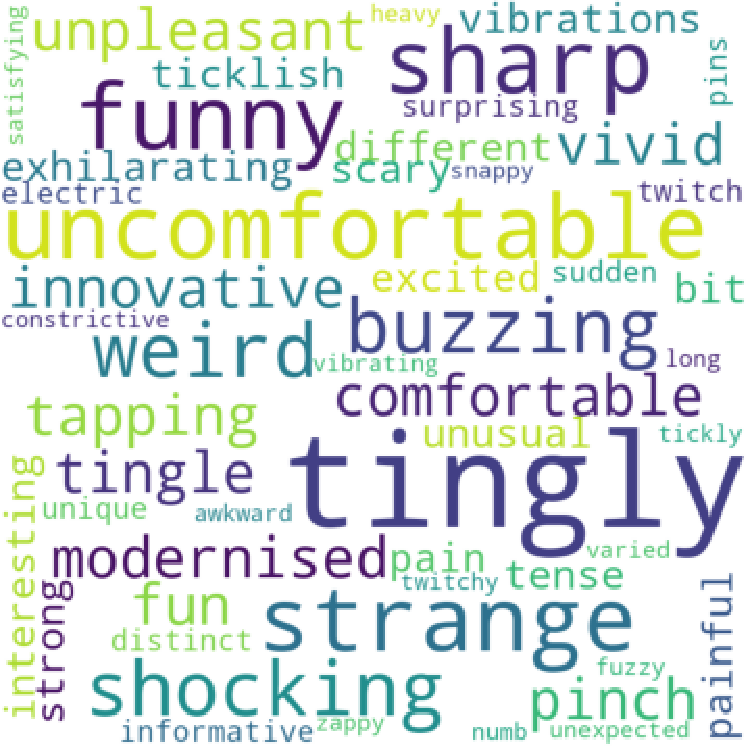
\includegraphics[scale=0.4]{images/wordmap.pdf}
    \caption{Word cloud highlighting common words used by subjects of the first two evaluations, describing the electrotactile sensation they experienced.}
    \label{fig:word-cloud}
\end{figure}

Interestingly, 'tingly' was the most common word used and was submitted a total of eight times. This equates to 11.5\% of all words obtained, meaning more than one in three people used this word to describe the electrotactile sensation. Other popular words included: 'funny', 'sharp', 'strange' and 'uncomfortable', all of which had three responses each. 

Performing sentiment analysis on these words was a good way to gather emotion on the subject. By looking at responses manually, we see that none of the popular words are especially positive, with most - namely 'tingly' - being neutral and some words, such as 'uncomfortable' being considered negative. We used Python's NLTK library \footnote{\url{https://www.nltk.org/}} to quantify an average happiness score across all words obtained. The calculated score would sit in a range between -1 (being extremely unhappy) and 1 (exceptionally happy). A score of -0.0872 was found from all words obtained, suggesting a slight unhappiness in responses. This is likely because participants were intentionally given a wide range of electrotactile signal strengths to choose from, some providing an unpleasant sensation. This also highlights the significance of research in this area, due to the poor experience electrotactile feedback offers if not configured carefully.\\

\subsubsection{Applications of Electrotactile Feedback}
Participants were asked to describe a situation where they could see electrotactile feedback being used in day-to-day life. The responses to this were varied with several users suggesting it would be useful when receiving notifications (\emph{"notifications"}, \emph{"Receiving notifications on your computer or other device"}, \emph{"Notifications from my phone"}). Other interesting suggestions included: when playing video games; using wearable devices, like smartwatches and VR headsets; and when using touchscreen keyboards (\emph{"Video Games as they develop more into VR etc."}, \emph{"Smartwatches"}, \emph{"When using touchscreen devices or other devices with no physical feedback like a keyboard"}).

\subsubsection{Summary}
The final question in the questionnaire asked users to summarise their thoughts on electrotactile feedback, based on their experience. Many of these summaries mentioned that as the signal became stronger it became more of an uncomfortable experience - reiterating the need for further refinement on the subject. \emph{"...when the tactile feedback was quite high it was worrying a bit and hurt a bit"}, \emph{"It is comfortable if the pulses are not too strong..."}, \emph{"...wasn't a big fan of the stronger settings however preset 2 and 3 were very good"}.

Positively, many of the summaries appeared to express interest in the area, suggesting they are keen to utilise electrotactile feedback after some refinement. \emph{"very fun to try"}, \emph{"It is definitely something that I am interested in seeing develop..."}, \emph{"Thought it was quite an enjoyable, new experience, not something I have done before"}.

Some responses, however, suggested they were not fond of the sensation and could not see themselves using the technology again. \emph{"Not something I completely enjoyed..."}, \emph{"I'm not sure I would use..."}.

\section{Evaluation Three: Keypad and\\Phrase Entry Tasks}
\subsection{Objectives and Hypotheses}
Having obtained promising results from the previous two quantitative evaluations, we decided it was beneficial to perform an additional, more qualitative, study. This was to gather a greater understanding of users' opinions of electrotactile feedback when performing more realistic tasks.

We also compared the time taken and accuracy of keystrokes as users completed tasks, with and without electrotactile feedback. This would give us a greater understanding of the wider impacts this feedback modality has on user performance.

\subsection{Design, Setup and Procedure}
Once again, a setup approach similar to before was maintained. The apparatus outlined in Section \ref{sec:apparaus} was again utilised and the same ethics procedure as before was followed (Section \ref{ethics}). Positioning of the self-adhesive electrodes was also consistent (Figure \ref{fig:hand}). This time, however, the instructions given to subjects differed. 

Participants were asked to complete four stages. First, a random six-digit number was displayed on the application window. By utilising the supplied mouse on a number pad which also appeared on the screen, subjects were instructed to enter this number as quickly and as accurately as possible. During this time, they were asked to keep their hand with the electrodes attached, flat on the table. They were required to enter ten numbers, without experiencing any electrotactile feedback. Following this they moved to the second stage, which was identical, other than electrotactile feedback being emitted from interaction with the keypad. The time taken for users to enter each number was recorded and so too were their keystrokes - this was to compute an accuracy metric.

During the third and fourth stages, phrases were selected at random from the set compiled by Mackenzie \cite{phrases_dataset}. The participants were then to type the selected phrase into a text input widget. As with the first two stages, their times and keystrokes were recorded, so they were advised once more to enter the phrases as quickly and as accurately as possible. Subjects again had to enter ten phrases without tactile feedback and then ten phrases with electrotactile feedback. We allowed participants to utilise both hands to type. While this may have introduced some unknowns, we determined it was more beneficial to maintain natural typing habits, as far as possible. This would lead to more accurate times and keystrokes being recorded. During the third stage no electrotactile feedback was experienced, whereas it was enabled for the fourth stage.

The strength of feedback provided to participants was based on the results of the second evaluation (section \ref{results-2}). Since the median presets were found to be the most popular among subjects here, these were chosen as the strengths for use in this evaluation. Due to the number entry stage consisting of users clicking buttons on the screen, the button preset was used (pulse-width: 92${\mu}s$, frequency: 56PPS, amplitude: 11mA). The phrase entry stage involved users typing text, similar to in prior studies, so the text widget preset was chosen (pulse-width: 97${\mu}s$, frequency: 49PPS, amplitude: 11mA).

Demonstration windows were shown to users before each of the four stages. The times and keystrokes were not recorded for these windows and existed to give users a break between the stages. They also allowed users to practice the stage they were about to commence.

The application (Section \ref{software-requirements}) was again modified to accommodate the requirements. The keypad used to enter numbers needed to be created from scratch, including the functionality of the buttons, including backspace. Methods of recording time and keystrokes also needed to be implemented, since these were being recorded in the results. Input validation was also a challenge, particularly for the phrase entry stages where users could potentially enter any character on the keyboard. We disabled users from using the arrow keys to change the position of the cursor. Clicking in the text box to change the cursor position was also disallowed, enforcing the use of the backspace key to fix mistakes.

Figure \ref{fig:gui-3} shows the interface presented to users for both number entry and phrase entry tasks.

\begin{figure}
    \centering
    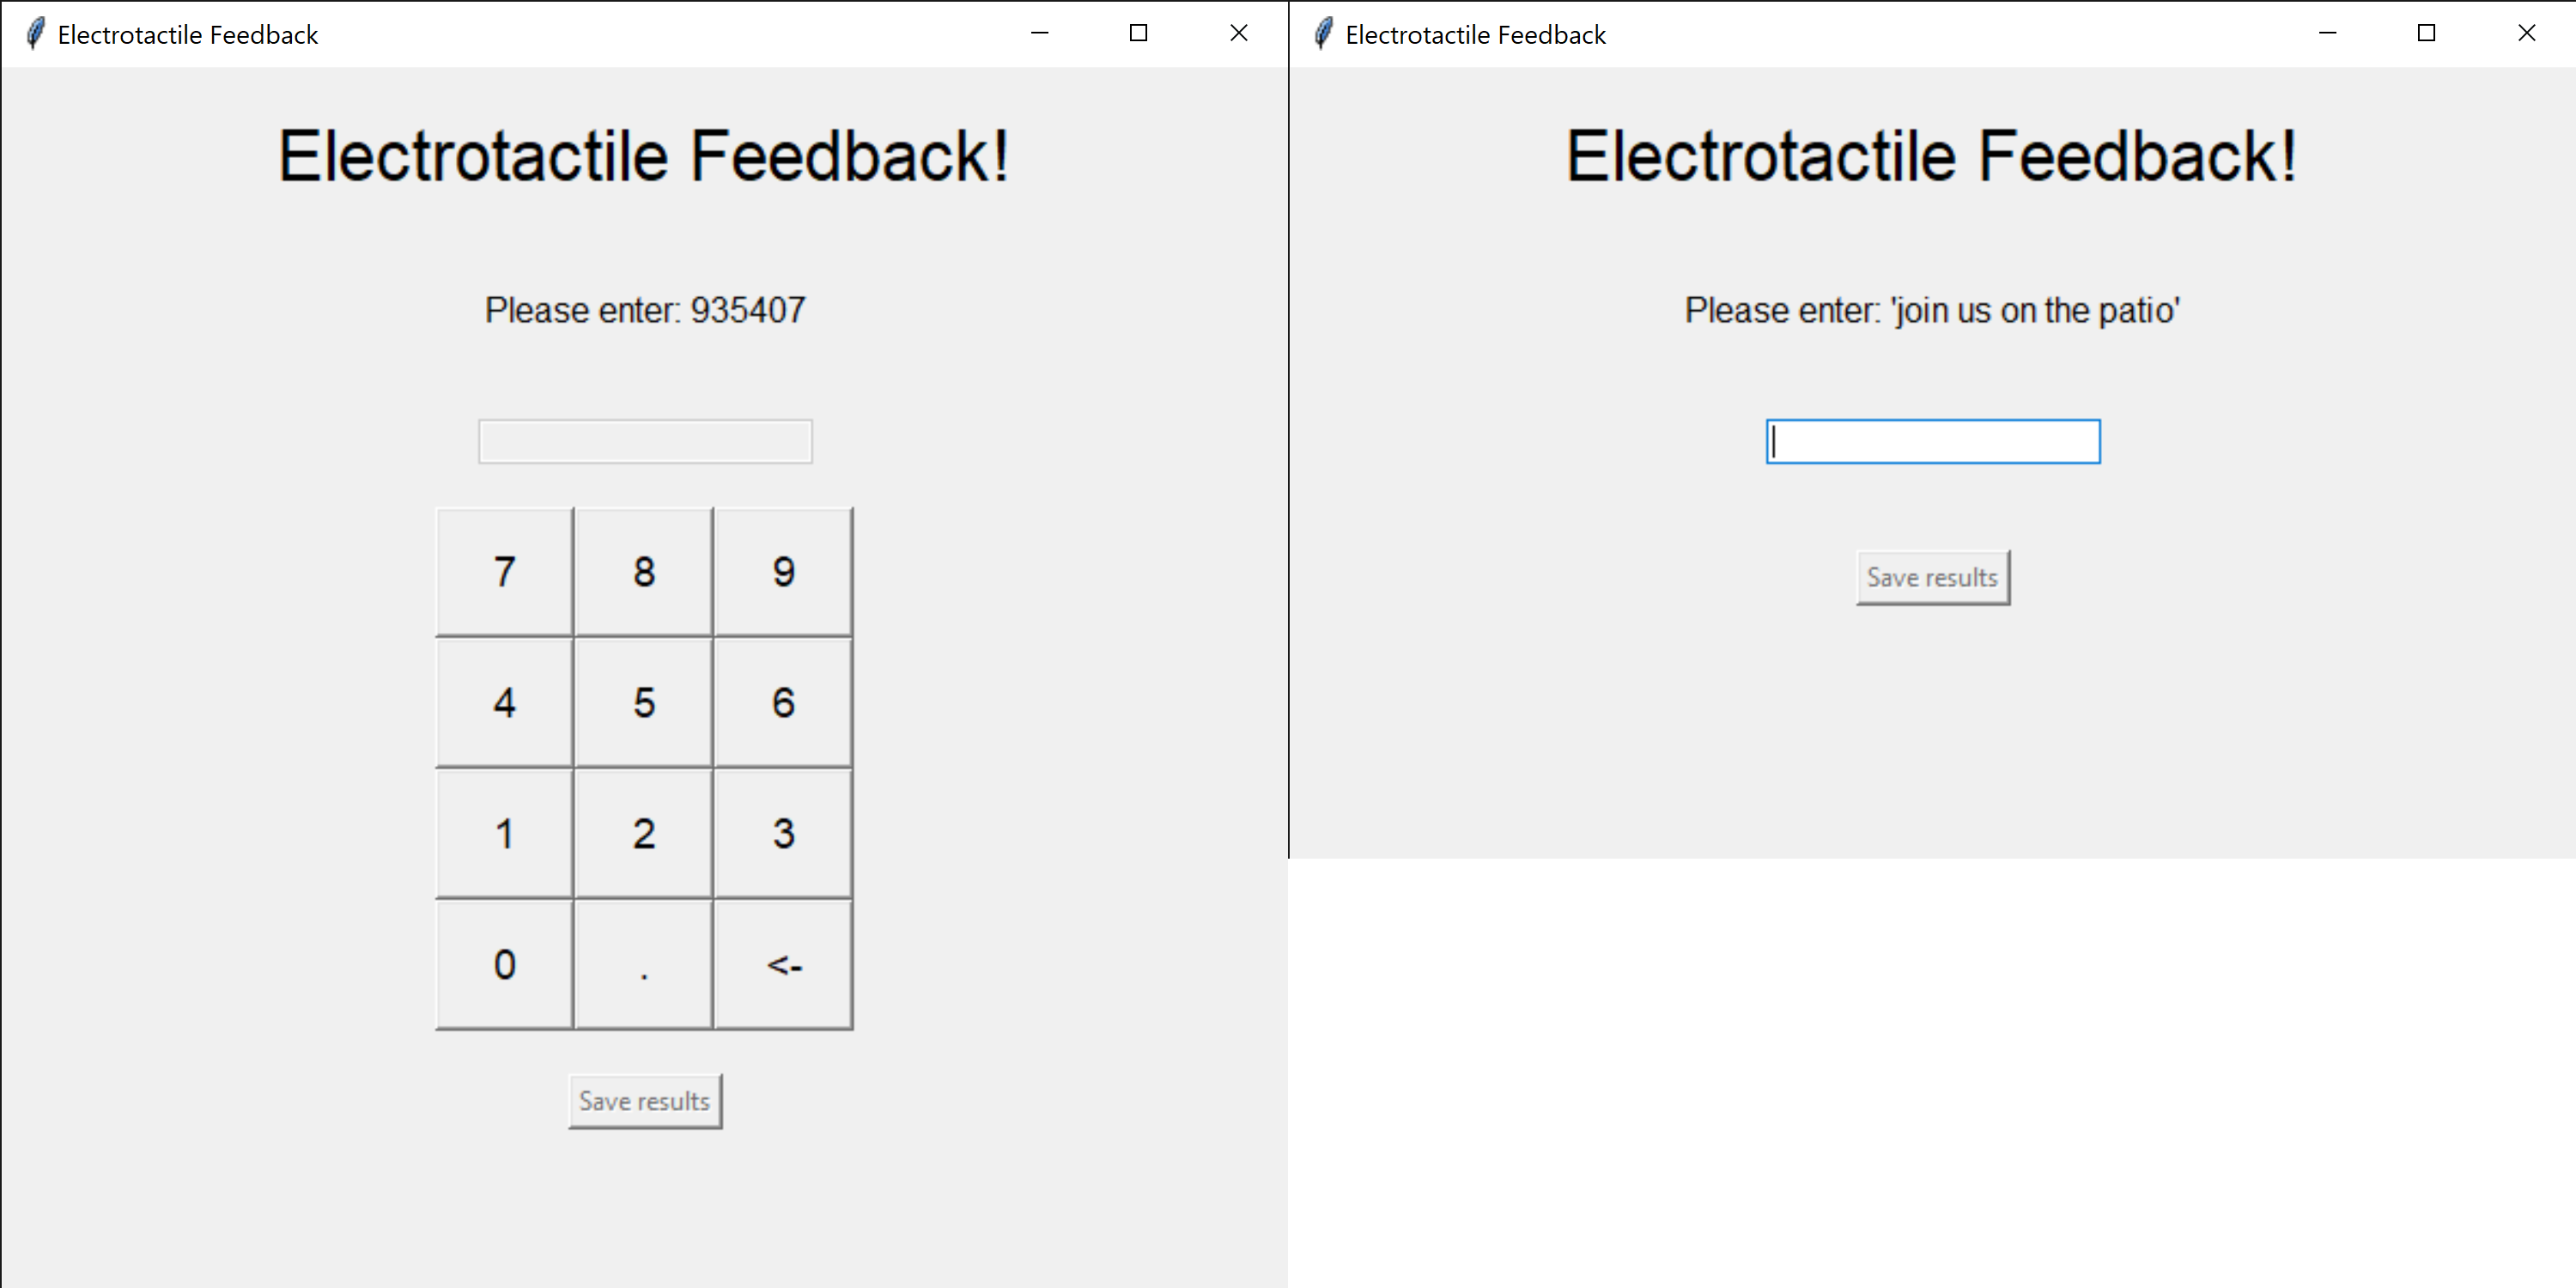
\includegraphics[scale=0.08]{images/Electrotactile Feedback 11_03_2024 13_55_31.png}
    \caption{Window displayed to users for number entry task (left) and phrase entry task (right).}
    \label{fig:gui-3}
\end{figure}

Upon completion of the tasks, users were given a questionnaire to answer. This questionnaire was more extensive than those prior and included numerous qualitative questions targeting the users' experience of electrotactile feedback. The results of this questionnaire were held separately from the previous two studies and are discussed in detail in section \ref{discussion-3}.

\subsubsection{Participants}\label{participants-3}
We allowed participants of our prior experiments to take part in this study. This was beneficial as it allowed us to ask users to compare their two experiences. Furthermore, allowing repeat users aided in recruitment and as a result, 14 participants signed up for this evaluation - nine of whom were involved with either one of our previous studies. Of these nine participants, three took part in phase one (Section \ref{sec:eval-1}) and the remainder in phase two (Section \ref{eval2}). 

Two of our participants were female and the remaining 12 were male. Six were in the 19-21 age group and eight were aged 22-25. Again, all participants were right-handed, so electrodes were again attached to the palms of left hands in all cases.

\subsection{Results}\label{results-3}

\begin{figure*}
    \centering
    \begin{subfigure}{0.45\textwidth}
        \includegraphics[width=\textwidth, page=3]{images/combinepdf.pdf}
        \caption{\% time decrease for keypad task.}
        \label{subfig:time-numpad}
    \end{subfigure} \hfill
    \begin{subfigure}{0.45\textwidth}
        \includegraphics[width=\textwidth, page=4]{images/combinepdf.pdf}
        \caption{\% time decrease for phrase entry task.}
    \end{subfigure} \hfill
    \begin{subfigure}{0.45\textwidth}
        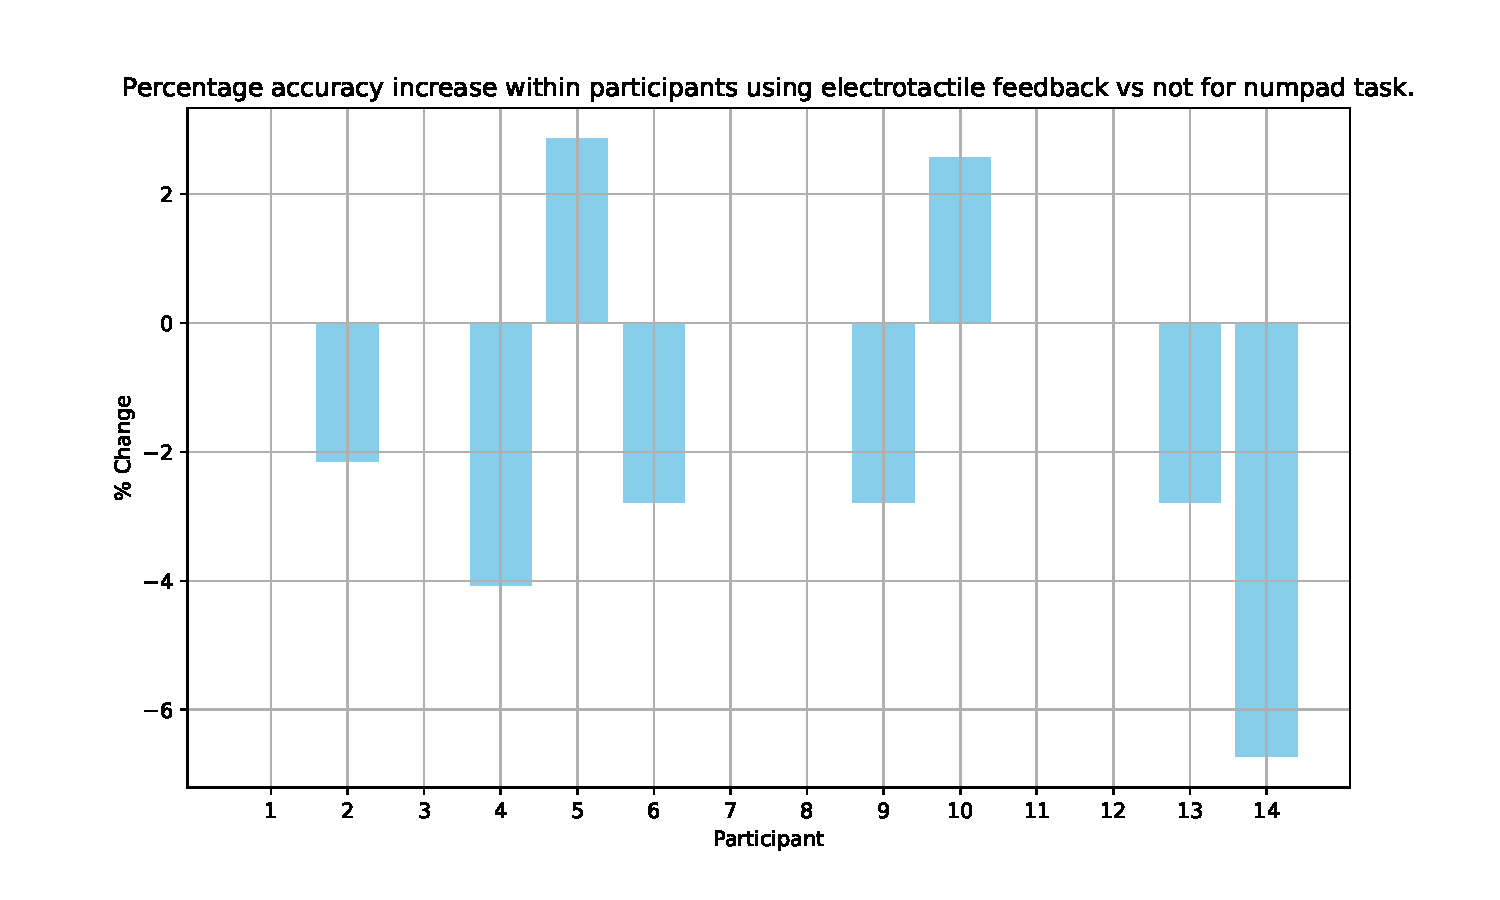
\includegraphics[width=\textwidth, page=1]{images/combinepdf.pdf}
        \caption{\% accuracy increase for keypad task.}
    \end{subfigure} \hfill
    \begin{subfigure}{0.45\textwidth}
        \includegraphics[width=\textwidth, page=2]{images/combinepdf.pdf}
        \caption{\% accuracy increase for phrase entry task.}
    \end{subfigure} \hfill
    \caption{Percentage difference in time and accuracy for each participant when performing keypad and phrase entry tasks, with and without electrotactile feedback.}
    \label{fig:percentage-changes}
\end{figure*}

Completion times were compared within users, meaning that we compared users to themselves - looking at the percentage difference in their response times with and without electrotactile feedback. We did not compare the raw times between users since some may be naturally slower at typing than others.

We first computed the mean and standard deviation in response times across all 10 responses, for each stage. Any responses where the times lay beyond two standard deviations of the average of the user, were excluded from calculations. This prevented entries where the user took particularly long from skewing our results. For both keypad entry and phrase typing tasks, the time difference was found between no-tactile and tactile times. It was returned as a negated percentage of the no-tactile time (negated to aid visualisation - a decrease in time equates to an increase in efficiency). Figure \ref{fig:percentage-changes} shows the percentage decrease in times, for both tasks, across each participant when utilising electrotactile feedback.

At this point, we calculated an average percentage time difference across every participant. Doing so revealed that subjects were on average 8.94\% faster when using electrotactile feedback for the number entry task and 6.23\% faster during the phrase entry task. An increase in efficiency was observed in 13 out of 14 cases for the keypad task (or 92.9\%) and 10 out of 14 in phrase entry tasks (71.4\%).

Accuracy was also considered. We again excluded from calculations, the responses which were faster or slower than two standard deviations of the user's average time. Thus, once again, preventing us from considering accuracies of oddities in responses. The accuracy score was calculated by taking the number of characters in the original phrase (including spaces) and dividing this by the number of characters entered by the user (including backspaces). Similar to the process undertaken for times, the average accuracy was then calculated for each participant, across each of the four stages. The difference was found between accuracies with and without electrotactile feedback and was multiplied by 100 to obtain a percentage. Bar plots showing the percentage difference in participant accuracy during both tasks are also shown in Figure \ref{fig:percentage-changes}.

Aggregating these results across every participant, we see that for the keypad task, the accuracy was found to decrease by approximately 1.13\%. Conversely, the phrase entry task displayed an accuracy increase of around 4.16\%. A decrease in accuracy was noted for six users (43\%) and two (14\%) being more accurate during the keypad entry task. The phrase entry task displayed an accuracy increase across eight users (57\%) and the remainder showed a decrease.

You can view these plots and the logic behind calculations, as well as some questionnaire analysis, in more detail, by referring to the third Jupyter Notebook file available on GitHub. \footnote{\url{https://github.com/AaronMilne19/electrotactile-feedback/blob/525683bfec8519a3c0c7227c2b925527da2b54a0/data/notebooks/electrotactile_results_phase3_analysis.ipynb}}

\subsection{Discussion}\label{discussion-3}
The results obtained demonstrate that participants respond faster on average when experiencing electrotactile feedback, than when not. In fact, regarding the number entry task (Figure \ref{subfig:time-numpad}), an increase in time was observed in only one case. There was a negligible change in accuracy for this task too - a decrease of only 1.13\% being observed. The accuracy for this task was, however, very high in general, with five participants scoring 100\% accuracy with and without tactile feedback. While these results represent a promising advantage to electrotactile feedback, it is important to mention some potential caveats with them. 

\subsubsection{Limitations of Time and Accuracy Metrics}
A potential area of bias in the times obtained is that on all occasions, participants performed both tasks with no feedback first. As participants became familiar with the challenge, they may have gathered momentum. Therefore, it is possible that the increase in efficiency observed could have come - at least in part - from this. A potential solution to this limitation could have been to randomise the situations where electrotactile feedback was enabled versus disabled.

This limitation affected the phrase entry task to a lesser extent. Since the phrases were randomly selected from a pre-established set, users would need to type new sentences each time - irrespective of the signal experienced. What could have impacted the times here, was the difficulty of specific phrases - some containing longer, more challenging words to spell. To minimise noise, specific phrases could have been manually selected and presented to every subject. This would have ensured phrases were consistent across participants, with and without electrotactile feedback.

Two bugs with the application were noticed when analysing the accuracy metrics of this study. The first was that the recording of the original phrases provided for users to type, to the results file, was overlooked. This meant that to compute an accuracy score, we had to reconstruct the original phrase, by parsing each user's response including backspaces. This issue on its own would not impact the scores, however, the second bug was brought to light during this process. The second bug occurred in the specific cases where the backspace character was pressed repeatedly by subjects (most likely held down for some time). The issue was that on some occasions, fewer backspace characters were saved to the results file than were pressed. A combination of the bugs meant that in the cases mentioned, not only was the number of recorded characters pressed by participants understated but on these occasions, the length of the reconstructed phrase would also have been overstated. Consequently, the accuracy scores obtained here were inflated.

Despite us recruiting a greater number of participants for this study than either of the previous, results would have been stronger had additional subjects taken part. 

\subsection{Questionnaire} \label{subsec:questionnaire-3}
The questionnaire provided to subjects upon completing the evaluation was critical to gathering qualitative opinions for our objective. This questionnaire asked some repeat questions, such as our 'provide three words' question. Responses were to be based exclusively on their experience with this study, not on any prior. Some new questions were also asked, like to rank the suitability of the perceived signal strength. Participants who had taken part in either of the previous studies were also asked additional questions designed to compare their experiences.

\subsubsection{General Thoughts}

Subjects were first asked to rate how much they enjoyed the electrotactile sensation they experienced, on a scale of 1 to 5 (5 being 'I loved it'). 50\% of the users selected options 4 or 5 here, suggesting that half of those asked either liked or loved the sensation. A further 28.6\% selected option 3 - implying they were quite neutral - and the remaining 21.4\% chose option 2, meaning they disliked the experience. No one responded with option 1, being that they hated the sensation.

Users were also asked if they believed the electrotactile signal impacted their times and accuracy. 64.3\% of participants believed that their times were similar, with and without feedback and 71.4\% thought the same of their accuracy. Interestingly, only 2 participants (14.3\%) believed the electrotactile signal made them faster at performing the tasks. This is surprising as it contradicts our findings that participants were on average faster. Three participants (21.4\%) thought that electrotactile feedback made them more accurate, which again is interesting since we found that accuracy was lesser impacted by the cues.

\subsubsection{Electrotactile Signal Strength}
Participants were asked to rate the strength of electrotactile feedback they received. Three users claimed the strength was too strong, six believed it to be just right and five believed the signal to be too weak. This aligns with the results shown in Figure \ref{fig:preset-results}, where the majority chose the median preset (the one experienced) and the stronger, preset 4, being preferred with the second most frequency. 

Subjects were then asked if the strength of feedback was suitable (comfortable and appropriate) for the type of interaction undertaken. This was on a scale from 1 (no) to 4 (yes). Four users selected option 4, another four selected 3, a further four selected 2 and only two users claimed it was not appropriate at all. This shows that 60\% of people found the preset more suitable than not - implying a good enough setting for their needs. When asked to explain their choice, many suggested that they found the strength suitable for either one of the tasks and slightly too weak or too strong for the other. For example, one participant wrote \emph{"numpad strength was suitable but text strength was too weak"}.

\subsubsection{Word Cloud}\label{subsubser:word-cloud-3}
Another word cloud was produced from the responses to the \emph{'provide three words'} question. Unlike with the first two studies, the responses here were kept separate, as we would like to compare the sentiment of words chosen after refinement of the feedback. Figure \ref{fig:wordcloud-3} shows the word cloud produced. Once again, 'tingly' was the top word used to describe the sensation with this being used on 5 occasions. 'tingle' was also used on two occasions, therefore of all 35 words, these made up 20\%.

\begin{figure}
    \centering
    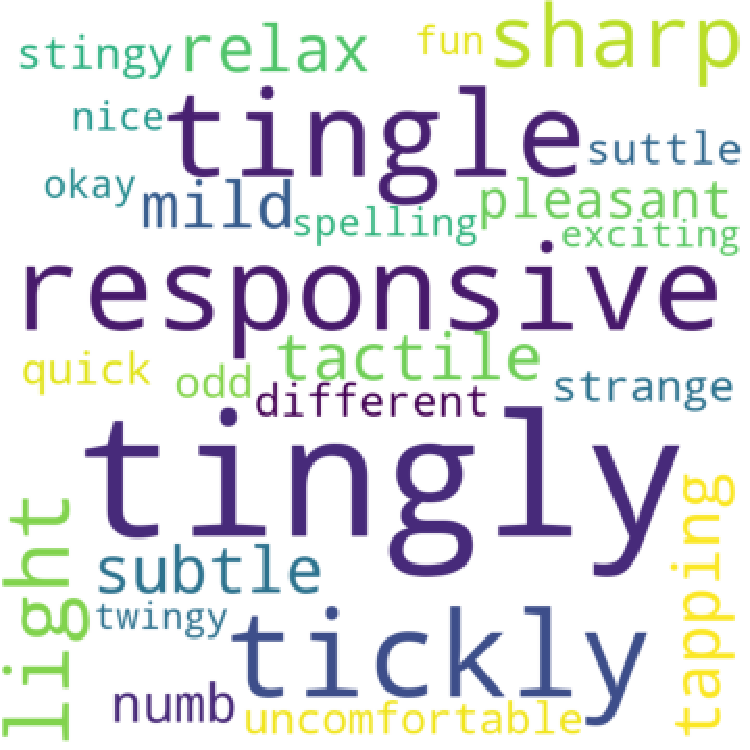
\includegraphics[scale=0.4]{images/Wordcloud-3.pdf}
    \caption{Word cloud highlighting common words used by subjects of the third study to describe the electrotactile sensation they experienced. }
    \label{fig:wordcloud-3}
\end{figure}

Sentiment analysis was again performed on the words, similar to before (Section \ref{subsec:questionnaire-1-2}). An average happiness score was computed to be -0.0144, suggesting words used to describe the electrotactile sensation, with our refinements, were almost neutral (1.4\% unhappy).

\subsubsection{Participants with Prior Experience}
Nine participants from one of the prior studies were included in this investigation. They were asked two supplementary questions, aimed at contrasting their experiences between the evaluations. First, participants were queried if they would have selected the same electrotactile signal setting experienced in the current study, had they encountered it in the previous one. Six out of the nine participants (66.6\%) affirmed they would have made this choice. Notably, this proportion exceeds that of participants who chose this preset initially in study two (Section \ref{results-2}).

Subsequently, they were asked to summarise how this experience compared to their previous. Here, some people mentioned that they liked the strength used this time and were not fond of the stronger settings from before. Others mentioned that the previous phase was \emph{"much better in terms of feeling the electrotactile feedback"}, suggesting that the strength was slightly too weak for them - once again highlighting the subjective nature of electrotactile perception.

\vfill\break
\subsubsection{Summary}
Users were again asked to summarise their thoughts on using electrotactile as a method of feedback. The key theme occurring across responses was mostly positive, with many highlighting the usefulness of electrotactile feedback in certain situations. Despite acknowledging some of the potential use cases, some of these respondents were still not enthusiastic about the feedback, as it was presented to them on the day.

To quote some direct summaries that highlight this theme: \emph{"Potentially useful, but not quite in the way utilised."}; \emph{"I felt it works well when you're typing as each keystroke is intentional, while for clicking you do it subconsciously and can be annoying"} and \emph{"I like it for clicking on buttons or submitting forms but not for typing as well"}.

\subsubsection{Limitations of Questionnaire Responses}
The questionnaire could have been improved by asking questions specific to the two tasks. Questions such as 'Was the strength suitable' or questions targeting times and accuracy, could also have appeared twice - specifying the task. This would have given us more granular responses. For example, if a participant believed the electrotactile feedback made them more accurate for typing tasks, but thought it made no difference to the number entry task, this setup would have allowed us to extract this information. 


\section{Overall Discussion} \label{overall-discussion}
\subsection{Recommendations}
Based on the insights gathered from our three evaluations, we propose the following as a starting point for electrotactile design:
\begin{itemize}
    \item Ideal electrotactile parameter settings are subjective and will differ between one user and the next. However, appropriate values for these will fall inside the optimal range discovered (pulse-width: 60${\mu}s$-130${\mu}s$, frequency: 30PPS-65PPS and amplitude: 9mA-15mA) in most cases.
    \item The median strength presets established, were found to be most popular among users, being chosen up to 55.6\% of the time during our second evaluation. They included:
    \begin{itemize}
        \item Pulse-width = 92${\mu}s$; Frequency = 56PPS; Amplitude = 11mA: for button interactions.
        \item Pulse-width = 97${\mu}s$; Frequency = 47PPS; Amplitude = 10mA: for radio button interactions.
        \item Pulse-width = 89${\mu}s$; Frequency = 49PPS; Amplitude = 11mA: for multiple-select interactions.
        \item Pulse-width = 97${\mu}s$; Frequency = 49PPS; Amplitude = 11mA: for text input interactions.
    \end{itemize}
    \item While these presets were the favourites, many found them too weak. Evidence of this is clear via the slightly more intense preset (preset 4) performing second best across all interaction types - being selected up to 33.3\% of times.
    \item Some users described the mentioned presets as being too strong and our results reflected this. A preset carrying a weaker perception (preset 2) was chosen on up to 16.67\% of occasions.
    \item These three presets (2, 3 and 4 - as detailed in Table \ref{tab:presets}) would, therefore, be considered appropriate starting options for users.
\end{itemize}

\subsection{Questionnaire Comparisons}
\subsubsection{Word Cloud Sentiment}
As discussed in sections \ref{subsubsec:word-cloud-1-2} and \ref{subsubser:word-cloud-3}, participants from all studies were asked to select three words that best described the electrotactile sensation they experienced. Word clouds were generated based on these words, and sentiment analysis was completed. The average happiness score derived from the responses of studies one and two was -0.0872, while the score from the final study was -0.0144. This reflects an 83.5\% increase in happiness observed in the third evaluation compared to the first two.

Due to the smaller pool of responses, fewer words were obtained during the third evaluation than from the first two. Consequently, the happiness score obtained from this evaluation may be less precise. Moreover, the absolute difference in happiness scores remains small, with neither score indicating extreme pleasure or distaste. The nature of the first two studies may also have led to an artificially low score being obtained there, as users were intentionally exposed to various strengths of feedback - some of which were likely uncomfortable. Despite this, the increase in happiness score demonstrates that the refinements made during this research made a noticeable improvement on user emotion of the topic. 

\subsubsection{Likelihood of Future Use}
A question was posed to participants across all evaluations. Based on their on-the-day experience, rate on a scale of 1 to 5, how likely it is they would use a refined version of electrotactile feedback in the future. During the first two studies, 39.1\% of people responded with option 3 or less - suggesting they are unlikely to use it again. However, during the final evaluation, only 28.6\% of participants out of the 14, responded with option 3 or less. This suggests that exposing participants to only a single, appropriately configured, signal for the interaction taking place, made a positive impact on user opinions on revisiting the technology. 

It is possible that applying electrotactile feedback to a realistic task also made a difference here. Previously, users were simply interacting with a superficial widget, so clarity in the applications of the feedback, may have been poor.

\subsubsection{Summaries}
Summaries obtained from the first two studies focus on users' initial impressions, novelty, and potential applications of electrotactile feedback. There's an emphasis on discomfort with the stronger signals. In contrast, those obtained from the final evaluation concentrate on individual preferences and the effectiveness of electrotactile feedback in enhancing accuracy. Both sets touched on the need for customisation, with the first two studies emphasising novelty and potential while the final study focuses more on user preferences and practicality.

Overall the summaries of the final study convey a slightly more positive outlook. Here, users express enjoyment and appreciation for the feedback during intentional actions like typing. There is also an acknowledgement of the utility and an expression of interest in future development. While some discomfort is mentioned, it appears to be balanced with positive remarks about the potential benefits and applications of electrotactile feedback.

\subsection{Areas for Future Research}
Through conducting our research, we have uncovered several areas which would benefit from further investigation. As mentioned in Section \ref{sec:intro}, Figure \ref{pulse-struc} shows two components of the electrotactile signal, where we did not place much focus: Pulse-Interval and Refresh Period. Future research, designed to uncover how these parameters also affect user perceptions of electrotactile feedback, would make a valuable contribution to the field.

Further analysis and fine-tuning of the popular presets we discovered would certainly be beneficial to the topic. Our results made clear that while our median presets were popular among participants, they were not appropriate for everyone, with many saying they were too weak or too strong. Tweaking the parameter values with more precision could lead to more pleasurable presets being discovered, enhancing the usability of electrotactile feedback.

Another area to mention would be the uncertainty regarding the threshold at which cues can be felt. This likely differs based on various factors, including the biology and conditions of the skin to which the electrodes are attached, as well as the physics behind how electrotactile signals operate. The desensitisation of users to the signals is also something which appears to affect this threshold and requires deeper analysis.

\section{Conclusions}
Throughout this paper, we completed three evaluations - each expanding on the results of the last. In the first study, we asked users to interact with four different widget types and to tune the strength of the electrotactile signal they experienced in the process. The results of this proved interesting as a clear cluster of values was obtained, indicating the presence of an optimal region of settings.

This finding was explored further in the second evaluation, where five presets were chosen deterministically from the previous study's results. Subjects were then to interact with the same four widget types as before, this time attempting all presets before deciding on their preferred one. The results showed that the median preset, was the clear victor across all widgets - reinforcing our theory of an optimal zone.

Finally, we looked more generally at users' thoughts on electrotactile feedback. By presenting a more realistic environment, users were given the task of inputting various numbers and phrases. They would experience electrotactile feedback for half of the entries and only visual feedback for the remaining half. Results showed not only an increase in efficiency when utilising electrotactile feedback but also that for many of the subjects, the strength of signal experienced was either just right for the task or close to it.

In conclusion, the findings indicate that there is still ample opportunity for continued investigation and improvement within the field. However, despite the need for further refinement, the results obtained are compelling. They imply that there isn't a one-size-fits-all solution when it comes to electrotactile signals, highlighting the necessity for customisable approaches in designing such systems in the future.

Moreover, the results suggest that while not everyone may be interested in this form of feedback at all, those who are should find a setting appropriate for them lying somewhere in the optimal domain of values obtained. Furthermore, they suggest that while individual preferences on stimuli remain specific, we have found a preset in this domain that up to 55.6\% find suitable and two additional ones that cover up to 33.3\% and 16.7\% of others. These presets will, therefore, form useful foundations for electrotactile feedback design in the future.

Finally, the opinions expressed by users when using the favoured preset in a practical setting appear positive, with plenty of interest being expressed in the technology. The change in sentiment after making the refinements outlined in this paper was also sizeable, indicating a prosperous future for electrotactile feedback, assuming the technology can be further refined and fine-tuned to work on an individual basis.

\vskip8pt \noindent
{\bf Acknowledgments.}
I would like to take the opportunity to thank everyone involved with this project, including all the participants who gave their time to partake in the above experiments. Most importantly my supervisor - Prof S. Brewster - who's guidance was critical to creating what you have just read. I would also like to extend a thank you to all who have supported me throughout this process; namely my family and friends, who have all provided the best encouragement I could have asked for.

\bibliographystyle{abbrv}
\bibliography{ElectrotactileFeedback}


\end{document}
